% IEEE Conference Paper - SIF Paper Draft
\documentclass[conference]{./template/IEEEtran}

\usepackage{cite}
\usepackage{amsmath,amssymb,amsfonts}
\usepackage{algorithmic}
\usepackage{graphicx}
\usepackage{textcomp}
\usepackage{xcolor}
\usepackage{tikz}
\usepackage{forest}
\usetikzlibrary{arrows.meta,positioning,shapes,calc,decorations.pathreplacing}
\usepackage{listings}
\usepackage{array}
\usepackage{booktabs}
\newcolumntype{C}[1]{>{\centering\arraybackslash}p{#1}}
\newcommand{\lightrule}{\noindent\textcolor{black!30}{\rule{0.97\columnwidth}{0.4pt}}}
\newlength{\vizsep}\setlength{\vizsep}{0.35cm}
\newlength{\vizseplg}\setlength{\vizseplg}{0.5cm}
\lstset{
  basicstyle=\ttfamily\small,
  keywordstyle=\bfseries,
  language=Python,
  frame=single,
  breaklines=true
}

\begin{document}

\title{Symbolic Execution is (Not Quite) All You Need\\{\normalsize Version 0.1.0}}

\author{
\IEEEauthorblockN{Sophie Smithburg}
}

\maketitle

\begin{abstract}
Given a programming language implementation running on a host machine and a grammar, you can use symbolic execution and formal ISA semantics as oracles to extract a formal labeled transition system that simulates the implementation's behavior.

In plain terms: You can automatically derive executable formal specs from implementations---no one writes specs, everyone writes implementations, but you can't prove things about implementations directly. This technique lets you get the spec from the implementation (given its grammar).
\end{abstract}

\begin{IEEEkeywords}
TODO add index terms
\end{IEEEkeywords}

%%%%%%%%%%%%%%%%%%%%%%%%%%%%%%%%%%%%%%%%%%%%%%%%%%%%%%%%%%%%%%%%%%%%%%%%%%%%%%%
\section{Introduction}
%%%%%%%%%%%%%%%%%%%%%%%%%%%%%%%%%%%%%%%%%%%%%%%%%%%%%%%%%%%%%%%%%%%%%%%%%%%%%%%

% SOURCE: intro-sources-and-draft.md:76-78 (Synthetic Draft - Sophie's words)
% Provenance: 100% Sophie's words from Bluesky threads
% Minor edits: "it's" -> "its", added "We", "in the form" (was "in form")

We can model a programming language executing on a host machine as a host labeled transition system $H$ which, after having been fed $\mathcal{I}$, the implementation, simulates $G$---this is to say the PL is $G$, its implementation is $\mathcal{I}$, and the host machine is $H$. If we observe a set of traces $\tau \in \mathcal{T}$ of executions of $G$ recorded at the level of $H$, we can use a specific algorithm to extract an LTS $G'$ that simulates $H_\mathcal{I}$.

In concrete terms, one can think of $H$ as something like x86 or ARM, and $\mathcal{I}$ as something like CPython or V8. This matters because in practice everyone builds implementations. No one writes specs, but you can't prove things about implementations directly for the most part, and you can about specs. So in order to have an effective ratchet in the sense of the LangSec 2017 Perry Metzger talk, we want to be able to get these specs for these implementations.

To prove $G'$ faithfully captures $G$, we would need $G$ in a formalism that shares the same proof basis as $G'$---but in practice, this is never the case. The problem we're trying to solve practically speaking is inferring $G'$ when no one cares to actually write out $G$, they're all focused on $\mathcal{I}$. So what we do instead is prove that $G'$ simulates $H_\mathcal{I}$, the LTS $H$ after executing $\mathcal{I}$, by way of quotienting over all the implementation details of $H$ that aren't causally controllable by way of inputs to $G$ in the form of program structure or codata.

%%%%%%%%%%%%%%%%%%%%%%%%%%%%%%%%%%%%%%%%%%%%%%%%%%%%%%%%%%%%%%%%%%%%%%%%%%%%%%%
\section{Notation}
%%%%%%%%%%%%%%%%%%%%%%%%%%%%%%%%%%%%%%%%%%%%%%%%%%%%%%%%%%%%%%%%%%%%%%%%%%%%%%%

\begin{itemize}
% === EXISTING NOTATION (from main.tex - Sophie wrote these) ===
\item $\Sigma$ is the concrete runtime space, and in our case, it is parametric over the definition of an ISA\@. It's basically the main memory, registers, CPU flags, any state that is documented for a particular CPU or host machine. In the more abstract view of a labeled transition system, which we focus on in this paper, $\Sigma$ is simply the state space of $H$.
\item $X$ is computed indirectly, but can be defined directly. $X$ is the set of all the state of the subsystem (like the programming language under analysis) that can be controlled by a program in that programming language. \textcolor{red}{In the mechanization, configurations are concretely the function type $\text{Dim} \to \text{Value}$: dimension-indexed observations of host state. The configuration space $X$ is the image of $\pi$ within this type.} It is possible to extend this in the future to include input by way of any predefined input channel, but modeling codata introduces non-determinism, which is out of scope for the current paper.
\item $\pi$ is the mapping from $\Sigma$ to $X$, which we get precisely by the indirect computation mechanism hinted at above.
\item $H$ is the host machine, it can be seen as an LTS or a bog standard ISA
\item $G$ is the true transition system, or notionally, what would be the specification of the programming language if the programming language were defined by the implementation? In some very real sense, a lot of programming languages are. Take, for example, C, Python, and the fact that it's been stated about the specifications in the Python enhancement proposal process and other documents in the standard that if one were to follow them, it's likely, without other guidance, they would end up with an entirely different language.
\item $\mathcal{I}$ is the programming language implementation under analysis
% H_I: Sophie's phrase "the LTS H after executing I" + Claude added "the host machine primed with the implementation"
\item $H_\mathcal{I}$ is the LTS $H$ after executing $\mathcal{I}$---i.e., an x86 machine after executing the CPython binary, or an ARM machine after executing a V8 implementation
\item $G'$ is the transition system we extract from traces $\tau \in \mathcal{T}$ of running $H_\mathcal{I}$, i.e.\ the host machine $H$ or host labeled transition system without loss of generality. Additionally, $G'$ is composed from $R$.
\item $\Gamma$ is the formal grammar for $\mathcal{I}$. \textcolor{red}{We assume $\Gamma$ is context-free; the approach may extend to some context-sensitive grammars, but we target the core case here.}
\item $\gamma \in \Gamma$ is a production in the grammar
\item $\text{holes}(\gamma)$ is the set of holes in production $\gamma$
\item $\kappa_h$ is the sentinel value for hole $h$ in production $\gamma$
\item $\mathcal{C}$ is a covering set of programs that enumerate all productions in $\Gamma$, and alternatives in each production, in a minimized way to be elaborated upon later
\item $\tau \in \mathcal{T}$ is a trace, or a sequence of states and labels for the transitions between them, generated when we run the host machine $H$ over the programming language implementation $\mathcal{I}$ and a program from $\mathcal{C}$, which implies all the values relevant to updates (it is of course more convenient when the values for updates are provided for us; we presume this, we think without loss of generality, but perhaps that's wrong!)
\item $\mathcal{T}$ is the set of all traces $\tau$
\item \textcolor{red}{A \textbf{Hole-to-Hole (HTH) block} is the maximal straight-line region of execution between two consecutive holes in evaluation order---see Appendix~\ref{app:hth} for visualizations}
\item \textcolor{red}{$L$ is the set of HTH labels; each $\ell = (\gamma_s, h_i, \gamma_d, h_j)$ identifies the transition from hole $h_i$ in production $\gamma_s$ to hole $h_j$ in production $\gamma_d$, where $h_i \in \text{holes}(\gamma_s)$ and $h_j \in \text{holes}(\gamma_d)$ are consecutive in evaluation order. In the common intra-production case, $\gamma_s = \gamma_d$; cross-production transitions have $\gamma_s \neq \gamma_d$}
\item \textcolor{red}{$\ell \in L$ is a label for a step in our transition system, identifying which HTH region the step corresponds to}
\item $R_\ell(x, x') := \text{Guard}_\ell(x) \land \text{Update}_\ell(x, x')$ summarizes the preconditions and state transformations for a step labeled $\ell$
\item $R = \{R_\ell\}_{\ell \in L}$ is the family of relational summaries over all HTH labels
\item $R^* = \bigcup_\ell R_\ell$ and its transitive closure

% === OBSERVATION + CONTROLLABILITY (from Lean mechanization) ===
\item \textcolor{red}{$\text{observe} : \Sigma \to \text{Dim} \to \text{Value}$ is the observation function mapping host states to per-dimension observable values. The projection $\pi$ is defined in terms of $\text{observe}$ by restricting to tracked dimensions $X$}
\item \textcolor{red}{\textbf{Observation faithfulness} ($h_\text{faithful}$): $\forall \sigma_1, \sigma_2.\; \sigma_1 \in \text{Reach}(H_\mathcal{I}) \implies (\forall d.\; \text{observe}(\sigma_1, d) = \text{observe}(\sigma_2, d)) \implies \sigma_1 = \sigma_2$. The observation function is injective on reachable states: any reachable host state is uniquely determined by its observations among all states, not just other reachable ones---$\sigma_2$ is unconstrained. This asymmetry is necessary because $\text{IsXControllable}$ quantifies over all states in the fiber $\pi^{-1}(\pi(\sigma))$, including unreachable ones. Two unreachable states need not be distinguished from each other. This is the key hypothesis enabling co-refinement convergence (Section~V).}
\item \textcolor{red}{\textbf{X-controllability.} A label $\ell$ is \emph{X-controllable} at state $\sigma$ if $\ell$ is enabled throughout the fiber $\pi^{-1}(\pi(\sigma))$---that is, every host state with the same projected configuration can take the transition. This formalizes the concept underlying $\text{Alt}(s)$: X-controllable transitions are those whose firing depends only on $X$-visible state.}

% === ORACLE NOTATION ===
% SOURCE: Sophie dictation 2026-01-10 (VERBATIM)
\item $\text{Reach}(H_\mathcal{I})$ is the set of reachable states in $H_\mathcal{I}$
\item \textcolor{red}{$\text{BStates}(\mathcal{I}) \subseteq \text{Reach}(H_\mathcal{I})$ is the set of \emph{all} reachable states with branching behavior---i.e., $s \in \text{BStates}(\mathcal{I})$ iff $|\text{Alt}(s)| > 1$. The branching oracle $O$ discovers these via symbolic execution combined with formal ISA semantics (e.g., K framework reachability logic), both operating at the $\Sigma$ level.}
% DRAFT: Alt(s) refined - all feasible outcomes reachable by modifying π(s)
\item \textcolor{red}{$\text{Alt}(s)$ is the set of \emph{all} feasible branch outcomes from state $s$ that are reachable by modifying $\pi(s)$. This is the completeness constraint: if outcome $o$ is achievable by changing $X$-state at $s$, then $o \in \text{Alt}(s)$. Branches depending on state outside $X$ are either implementation-internal (irrelevant to $G'$) or trigger $\pi$-refinement to include that state.}
% DRAFT: O(s) produces constraints over π to achieve alternatives
\item \textcolor{red}{$O(s)$ is the branching oracle: given $s \in \text{BStates}(\mathcal{I})$, it produces constraints over $\pi(s)$ that achieve each alternative in $\text{Alt}(s)$}
% DRAFT: ReplayApply applies constraint to π, runs to get branch outcome
\item \textcolor{red}{$\text{ReplayApply}(s, c) \Downarrow o$ means replaying from state $s$ with $\pi(s)$ modified by constraint $c$ realizes branch outcome $o$}
% DRAFT: O* is fixpoint of both traces AND π refinement - up to behavioral equivalence
\item \textcolor{red}{$O^*(\mathcal{T})$ is the fixpoint up to behavioral equivalence: for each branch outcome $o \in \text{Alt}(s)$ at each $s$ along traces in $O^*(\mathcal{T})$, we require \emph{at least one exemplar trace} realizing $o$. We do not generate all traces---only one representative per behavioral pattern (same control flow, same HTH structure). Additionally, $\pi$ has stabilized. This suffices for completeness: every reachable behavior has an exemplar from which we extract $R_\ell$.}

% === SIMULATION ===
% SOURCE: Sophie dictation 2026-01-10 (VERBATIM)
\item $G' \preceq M$ states that $G'$ simulates $M$, which is to say that all behaviors of $M$ have corresponding behaviors in $G'$
\end{itemize}

%%%%%%%%%%%%%%%%%%%%%%%%%%%%%%%%%%%%%%%%%%%%%%%%%%%%%%%%%%%%%%%%%%%%%%%%%%%%%%%
\section{Main Claim}
%%%%%%%%%%%%%%%%%%%%%%%%%%%%%%%%%%%%%%%%%%%%%%%%%%%%%%%%%%%%%%%%%%%%%%%%%%%%%%%

% SOURCE: intro-sources-and-draft.md:82 (Sophie's words)
% Provenance: 100% Sophie's words from Bluesky

We reconstruct behavior piecewise along traces and each trace is a sound reconstruction because it almost literally replays the trace we saw. And also we use a model of the host machine that knows about branches to achieve completeness by adding new traces for all uncovered paths. If you manage soundness and completeness of reconstruction that's basically the whole game.

\subsection{Oracles}

\textcolor{red}{We require two kinds of oracles: one for branching behavior and one for value transformations. Neither is counterfactual---both are instantiated by real tools.}

\subsubsection{Branching}

The branching oracles we require are in no way counterfactual. Some aspects are partially captured by symbolic execution and then the rest of that is fully captured by formal ISA semantics.
\textcolor{red}{Throughout this paper, the ``branching oracle $O$'' refers to this combined realization---selective symbolic execution for path feasibility plus formal ISA semantics for reachability---not an additional assumption beyond symex. We use $O$ as notational shorthand.}

\paragraph{\textcolor{red}{Completeness.}}
% SOURCE: ChatGPT axiom screenshot, formalizing Sophie's "completeness by covering all branches"
\textcolor{red}{For all $\mathcal{I}$-relevant branch states and all feasible outcomes, the oracle can produce a constraint that achieves that outcome:}
\[
\textcolor{red}{\forall s \in \text{BStates}(\mathcal{I}).\; \forall o \in \text{Alt}(s).\; \exists c \in O(s).\; \text{ReplayApply}(s, c) \Downarrow o}
\]

\subsubsection{Value Transformation}

What we need for value transformation inference is provided fully by symbolic execution engines. \textcolor{red}{When symbolically executing a basic block, the engine produces symbolic expressions showing how input values map to output values---this directly gives us the $\text{Update}(x, x')$ component of each $R_\ell$.}

\subsection{\textcolor{red}{Proof Structure}}

\begin{enumerate}
\item \textcolor{red}{\textbf{Given}: $H$ (host), $\mathcal{I}$ (implementation), $\Gamma$ (grammar)}
\item \textcolor{red}{\textbf{Given}: $O$ (branching oracle)---instantiated by SSE or formal ISA semantics}
\item \textcolor{red}{\textbf{Define}: $\mathcal{T}_0$ = initial traces from covering set $\mathcal{C}$}
\item \textcolor{red}{\textbf{Define}: $O^*(\mathcal{T}_0)$ = fixpoint (apply $O$ until no new traces)}
\item \textcolor{red}{\textbf{Assume}: Symbolic execution recovers $\text{Guard} \land \text{Update}$ from HTH regions}
\item \textcolor{red}{\textbf{Construct}: $G'$ from $\{R_\ell \mid \ell \text{ derived from } O^*(\mathcal{T}_0)\}$}
\item \textcolor{red}{\textbf{Prove}: $G' \preceq H_\mathcal{I}$}
\end{enumerate}

\subsection{Soundness and Completeness}

\paragraph{Soundness.} Each $R_\ell$ is computed as the relational transformer associated with a hole-to-hole basic block. Our relational transformer is as sound as the symbolic execution engine we use to compute said transformer.

\paragraph{Completeness.} This follows basically from the definition of the branching oracle and the fixpoint. Since by definition the branching oracle can detect all branching behavior at the level of $H$, were there to be any state reachable in $H_\mathcal{I}$ that we did not find at least one exemplar trace for, then it's a contradiction with the assumption that the oracle is complete. \textcolor{red}{This is conditional on oracle completeness (symex being biconditional with $H_\mathcal{I}.\text{step}$); given this, the bisimulation Corollary (Section~V-E, \texttt{extraction\_bisimulation}) formally establishes both simulation directions, ensuring no reachable behavior is missed.}

\subsection{Scope of This Paper}

This current paper attempts to prove that it is possible to do such a reconstruction. We leave it for future work to fully implement such an algorithm and prove it correct. We don't consider it necessary to prove that the oracles exist because they do in the form of formal specifications of ISAs and symbolic execution engines. Our intent is simply to prove that, given such tools, it should be possible to extract semantics from the implementations and an algorithm corresponding to this sketch.

% SOURCE: Sophie dictation 2026-01-10 (VERBATIM)

We're only focused on ISAs, like Industrial ISAs, running industrial programming languages. We are not yet aiming to tackle them in their full generality, but rather to model as large of a slice of an industrial implementation as is possible. To this end, we make some radical choices in terms of scope to make proving any result possible, knowing that we must return to each of these in future work.

Out of scope for this paper are:
\begin{itemize}
\item non-determinism
\item concurrency
\item lazy evaluation
\item typing or any static analysis or codata
\end{itemize}

Each of these scope limitations would likely warrant their own follow-up paper in themselves. All of that being said, we think that this is still useful work, as the core semantics of a large class of industrially interesting programming languages can be captured this way.

%%%%%%%%%%%%%%%%%%%%%%%%%%%%%%%%%%%%%%%%%%%%%%%%%%%%%%%%%%%%%%%%%%%%%%%%%%%%%%%
\section{Methodology}
%%%%%%%%%%%%%%%%%%%%%%%%%%%%%%%%%%%%%%%%%%%%%%%%%%%%%%%%%%%%%%%%%%%%%%%%%%%%%%%

% SOURCE: Sophie dictation 2026-01-10

We use sentinels $\kappa_h$ in templates $P \in \mathcal{C}$ to determine the correspondence from a program with a particular AST construct executing and the resulting trace---particularly the mapping from sentinel holes to their corresponding values in the trace. We use this both to learn a mapping from syntactic representation to runtime representation, as well as to delineate the bounds of hole-to-hole basic blocks.

\subsection{Structured Programming and Lexical Scope}

\textcolor{red}{[NOTE: Sophie flagged this may need to move earlier]}

To explain what a hole-to-hole basic block is, we must first introduce the requirement of lexical scope in structured programming languages. Structured programming is necessary because it gives us the property that jumps are always lexically bounded with respect to the AST. For $\kappa_{h_1}$ to $\kappa_{h_2}$, that basic block, we identify the points in the trace that correspond to that. From those points in the trace, we can extract information like memory regions to feed to a selective symbolic execution engine to selectively symbolically execute just that region between those two holes.

\subsection{Learning the Configuration}

We are also using this to learn $\pi$. The idea is that we learn what our configuration should look like. Our configuration is defined by the bindings from AST paths to runtime values, so if something isn't AST-bindable or AST-referable, then it can't end up in our projection $\pi$.

\textcolor{red}{\textbf{Differential causality testing.} To learn $\pi$ concretely, we run paired experiments. For each hole $h$ in template $P$, we execute $P$ with two different sentinel values: $P[h \leftarrow \kappa_1]$ and $P[h \leftarrow \kappa_2]$. Comparing the resulting traces $\tau_1$ and $\tau_2$, we identify the positions where they differ. These differing positions represent state that is \emph{causally influenced} by the value at hole $h$---and therefore must be included in $X$.}

\textcolor{red}{The key insight is that $X$ is exactly the \emph{transitive closure of AST-bound state}. Nothing enters $X$ without first being directly bound to an AST position (by determinism---all state changes trace back to program structure). A variable's value is in $X$ because it was assigned from an expression; that expression's value is in $X$ because it was computed from subexpressions bound to AST nodes; and so on. The differential test reveals this transitive closure: if changing a sentinel at hole $h$ eventually affects some state $S$ in the trace, then $S$ is transitively reachable from $h$'s AST binding, and belongs in $X$.}


\subsection{Control Flow and Value Transformation}

We extract control flow and value transformation along this same part of the technique. The selective symbolic execution gives us path constraints. Say we're doing the if-then-else situation where we are going from \texttt{cond} to the then-branch. We'll have a path constraint induced by this that \texttt{cond} must evaluate to something truthy. We can flip that path constraint, and that gives us the other thing we have to explore. We would have already gotten that by way of our covering set in the case of truthy and falsy---at least for literal \texttt{true} and \texttt{false} we would have. What's key is that we get an SMT formulation in terms of things we have determined bindings for in terms of our AST---we've extracted the guard conditions for our labeled transition system.

For value inference: since these hole-to-hole blocks do not involve branching, we can extract the relational transformer along this basic block. We use the symbolic statement of inputs in the configuration mapping to symbolic expressions in the output. We can use those, plus the mapping from syntactic literal to runtime type, to define the value transformation aspect of semantics.

\subsection{\textcolor{red}{Bootstrapping and Co-Refinement}}

\textcolor{red}{\textbf{The boundary detection problem.} Finding HTH regions requires knowing where each hole's computation ``happens'' in the trace. But we cannot simply look for where sentinel \emph{values} appear---values can be inlined, constant-folded, or otherwise transformed by the implementation. We need to detect where \emph{computation} happens, not just where values appear.}

\textcolor{red}{Moreover, we cannot use syntactic heuristics like ``this AST node is named \texttt{if}'' or ``this node has two children.'' The entire point is to infer semantics from implementation behavior. If we hardcode syntactic patterns, we assume what we are trying to learn.}

\textcolor{red}{\textbf{Sentinel expressions.} Instead of sentinel values, we use sentinel \emph{expressions} that force observable computation---e.g., \texttt{(x := sentinel; sentinel)} where the assignment leaves a trace signature. When the assignment appears in the trace, we know that hole was evaluated. But to design such expressions, we must know which operations have observable sequencing.}

\textcolor{red}{\textbf{Learning algebraic laws from $R_\ell$.} Here is the key insight: $R_\ell$ is an SMT formula produced by symbolic execution. SMT formulas use SMT-LIB operations: \texttt{bvadd}, \texttt{bvmul}, \texttt{store}, etc. These operations have \emph{precisely defined algebraic laws}---this is the SMT-LIB standard. We do not pattern-match against heuristics; we read exact algebraic properties from the formula structure to identify what \emph{weakens} ordering detection:}
\begin{itemize}
\item \textcolor{red}{$R_\ell$ contains \texttt{bvadd}$(x, y)$ $\Rightarrow$ commutative $\Rightarrow$ \emph{cannot} use this to detect evaluation order}
\item \textcolor{red}{$R_\ell$ contains \texttt{bvsub}$(x, y)$ $\Rightarrow$ non-commutative $\Rightarrow$ \emph{can} use this to detect order}
\item \textcolor{red}{$R_\ell$ contains \texttt{store} $\Rightarrow$ has observable side effects $\Rightarrow$ \emph{can} use this to detect order}
\end{itemize}

\textcolor{red}{\textbf{Sequencing analysis.} Commutative operations cannot detect evaluation order: if $a + b = b + a$, we cannot tell from the result whether $a$ or $b$ was evaluated first. Non-commutative operations and side effects \emph{can} detect order. By reading the algebraic laws from $R_\ell$, we identify which operations are safe for sequencing detection.}

\textcolor{red}{\textbf{The bootstrapping loop.} This creates a productive cycle:}
\begin{enumerate}
\item \textcolor{red}{Start with rough HTH regions from initial trace differences and observable side effects}
\item \textcolor{red}{Extract $R_\ell$ via selective symex on each region}
\item \textcolor{red}{Read algebraic laws from $R_\ell$ (exact, from SMT-LIB operations)}
\item \textcolor{red}{Use laws to refine sequencing analysis---design better sentinel expressions}
\item \textcolor{red}{Get more precise HTH boundaries}
\item \textcolor{red}{Extract more precise $R_\ell$}
\item \textcolor{red}{Repeat until fixpoint}
\end{enumerate}

\textcolor{red}{\textbf{Convergence.} This process terminates because: (1) the grammar $\Gamma$ is finite, so there are finitely many operations to analyze; (2) algebraic law knowledge is monotonic---we only learn new laws, never unlearn; (3) HTH precision increases or stays the same with each iteration. The fixpoint is reached when no new algebraic knowledge yields more precise boundaries.}

\textcolor{red}{\textbf{Three-way co-refinement.} The full technique involves co-refinement across three dimensions:}
\begin{enumerate}
\item \textcolor{red}{\textbf{Configuration refinement ($\pi$):} Learning what state is program-relevant by observing causal influence of sentinels}
\item \textcolor{red}{\textbf{Region refinement (HTH):} Learning computation boundaries using sequencing-sensitive expressions, identified by their non-commutative semantics}
\item \textcolor{red}{\textbf{Semantic refinement ($R_\ell$):} Extracting relational transformers via selective symex, which reveals algebraic properties that inform sequencing detection}
\end{enumerate}
\textcolor{red}{These three refine together: better $\pi$ $\rightarrow$ better HTH detection $\rightarrow$ better $R_\ell$ $\rightarrow$ better algebraic knowledge $\rightarrow$ better HTH $\rightarrow$ \ldots\ until all three stabilize together with $O^*$.}

\subsection{Soundness and Completeness of the Technique}

This gives us a representation of individual paths that is as sound as either our symex engine and/or our formal semantics, to the extent we depend on either of those oracles and/or both. It is complete as both of those oracles as well. Since it's lexical scope, we don't have to do any scope inference. \textcolor{red}{[That's the whole technique.]}

%%%%%%%%%%%%%%%%%%%%%%%%%%%%%%%%%%%%%%%%%%%%%%%%%%%%%%%%%%%%%%%%%%%%%%%%%%%%%%%
\section{Proof}
%%%%%%%%%%%%%%%%%%%%%%%%%%%%%%%%%%%%%%%%%%%%%%%%%%%%%%%%%%%%%%%%%%%%%%%%%%%%%%%

% DRAFT: Claude's synthesis from notes_2026-01-10, notation-and-proof-synthesis.md, project_update_ideas.md
% This is a conditional result: guarantees are oracle-relative and scope-limited

\textcolor{red}{This section proves a conditional result: given a sound oracle for symbolic execution (subsuming grammar coverage, control-flow branching, and value transformation---see Section~V-A), the reconstructed semantics $G'$ simulates $H_\mathcal{I}$ within the constrained semantic domain defined in the Scope section. With the additional hypothesis that the oracle is also complete, we obtain bisimulation (Corollary~\ref{cor:bisim}).}

\textcolor{red}{\subsection{Oracle Decomposition}}

\textcolor{red}{We decompose the reconstruction's correctness into three oracle dependencies:}

\begin{enumerate}
\item \textcolor{red}{\textbf{Grammar oracle} ($\Gamma$): Provides full syntactic coverage of the language fragment. This may be a known grammar or one inferred via grammar-mining techniques. The grammar oracle delimits the syntax space but is not a source of semantic uncertainty.}

\item \textcolor{red}{\textbf{Branching oracle} ($O$, Section~III-A): The critical completeness dependency. We require \emph{local completeness} over branching behavior relevant to each reconstructed HTH region. The combined symex+ISA oracle (Section~III-A) serves as a branching discriminator, ensuring all feasible successor regions for a given syntactic construct are discovered.}

\item \textcolor{red}{\textbf{Value-transformation oracle}: Provides relational transformers $R_\ell(x, x')$ for basic blocks. May be instantiated by symbolic execution, relational symbolic execution, or trusted formal ISA semantics. This oracle primarily affects soundness: incorrect transformers yield unusable semantics, while partial transformers under-approximate behavior.}
\end{enumerate}

\textcolor{red}{In the Lean mechanization, the branching and value-transformation oracles are unified into a single parameter $\text{symex} : L \to \Sigma \to \Sigma \to \text{Prop}$, which soundly approximates $H_\mathcal{I}$'s transition relation. The existential projection of symex through $\pi$ captures both guard conditions (via the domain of the projected relation) and value updates (via its codomain). The grammar oracle is a structural precondition (\texttt{GrammarConformant}), not a runtime parameter. The three-way decomposition above is conceptual; the mechanization shows that a single sound symex oracle suffices.}

\textcolor{red}{\subsection{Setup}}

\textcolor{red}{Fix a host machine $H$, implementation $\mathcal{I}$, and grammar $\Gamma$. Let:}
\begin{itemize}
\item \textcolor{red}{$\mathcal{C}$ be a covering set of programs that exercises every production in $\Gamma$}
\item \textcolor{red}{$\mathcal{T}_0 = \{\tau_P \mid P \in \mathcal{C}\}$ be the initial traces from executing $\mathcal{C}$ on $H_\mathcal{I}$}
\item \textcolor{red}{$O$ be the symex+ISA oracle (Section~III-A) satisfying the completeness axiom}
\item \textcolor{red}{$O^*(\mathcal{T}_0)$ be the fixpoint of applying $O$ to traces until no new traces are discovered and $\pi$ has stabilized}
\end{itemize}

\textcolor{red}{\textbf{Labeling HTH regions (precondition).} HTH labels are assigned by construction in the template setting, not inferred from arbitrary program traces: each template exercises a single production with sentinels at holes, and the trace segment between consecutive sentinel evaluations defines the HTH block whose label is determined by template structure and observed evaluation order.
Concretely, each template $P \in \mathcal{C}$ is derived from some production $\gamma \in \Gamma$. The trace region between the computation of hole $h_i$ and hole $h_j$---where $h_i$ and $h_j$ are consecutive in that trace's evaluation order---constitutes an HTH region, and we assign it the label $\ell = (\gamma_s, h_i, \gamma_d, h_j)$ where $\gamma_s$ is the production containing $h_i$ and $\gamma_d$ is the production containing $h_j$ (typically $\gamma_s = \gamma_d$). For traces generated by exploring branches, different control flow paths may reach different holes, yielding different labels. The mechanism for detecting these boundaries---using sentinel expressions refined via algebraic laws---is described in Section~IV-D.}\footnote{\textcolor{red}{In lazy languages, demand patterns determine which holes are evaluated and when, introducing completeness concerns that sentinels and symbolic execution cannot address---one would need to instrument demand propagation itself. This is why we restrict to eager evaluation.}}

\textcolor{red}{For each trace $\tau \in O^*(\mathcal{T}_0)$, the value-transformation oracle produces relational summaries $R_\ell(x, x') := \text{Guard}_\ell(x) \land \text{Update}_\ell(x, x')$ for each HTH region labeled $\ell$ within $\tau$.}

\textcolor{red}{Define $G' := \langle X, L, \{R_\ell\}_{\ell \in L}, s_0 \rangle$ where:}
\begin{itemize}
\item \textcolor{red}{$X$ is the learned configuration space (the image of $\pi$)}
\item \textcolor{red}{$L$ is the set of HTH labels (see Notation)}
\item \textcolor{red}{$s_0 = \pi(\sigma_0)$ for some initial $H_\mathcal{I}$ state $\sigma_0$}
\end{itemize}

\textcolor{red}{\subsection{Co-Refinement Fixpoint}}

\textcolor{red}{\textbf{Definition} (Co-Refinement Fixpoint). The triple $(H_\mathcal{I}, \pi, R)$ satisfies the \emph{co-refinement fixpoint condition} if:}
\begin{enumerate}
\item \textcolor{red}{\textbf{Oracle soundness}: every concrete transition is captured---$\forall \sigma, \sigma', \ell.\; \sigma \xrightarrow{\ell} \sigma' \implies R_\ell(\pi(\sigma), \pi(\sigma'))$}
\item \textcolor{red}{\textbf{Non-controllable preservation}: non-X-controllable transitions from reachable states preserve the projection---$\forall \sigma, \sigma', \ell.\; \sigma \in \text{Reach}(H_\mathcal{I}) \land \sigma \xrightarrow{\ell} \sigma' \land \neg\text{IsXControllable}(\sigma, \ell) \implies \pi(\sigma) = \pi(\sigma')$}
\end{enumerate}
\textcolor{red}{Together these ensure the extracted LTS faithfully represents $H_\mathcal{I}$'s behavior at the granularity captured by $\pi$: observable transitions are in $R$'s domain, and unobservable transitions don't change the projected state.}

\textcolor{red}{\subsection{Extraction Construction}}

\textcolor{red}{We construct a concrete co-refinement process whose fixpoint yields $\pi$ and $R$ satisfying the conditions above. The construction uses three components:}

\begin{itemize}
\item \textcolor{red}{\textbf{Projection.} For a tracked dimension set $X \subseteq \text{Dim}$, define $\pi_X(\sigma)(d) = \text{observe}(\sigma, d)$ if $d \in X$, else a default value. Two states have the same projected configuration iff they agree on all tracked dimensions. The configuration type is $\text{Dim} \to \text{Value}$, so configurations are equal iff they agree on every dimension---tracked dimensions carry observed state, while untracked dimensions are padded with a fixed default.}

\item \textcolor{red}{\textbf{Oracle.} Given a symbolic execution oracle $\text{symex} : L \to \Sigma \to \Sigma \to \text{Prop}$ that soundly approximates $H_\mathcal{I}$'s transitions ($\forall \sigma, \sigma', \ell.\; \sigma \xrightarrow{\ell} \sigma' \implies \text{symex}(\ell, \sigma, \sigma')$), define $R_\ell^X(x, x') \iff \exists \sigma, \sigma'.\; \pi_X(\sigma) = x \land \text{symex}(\ell, \sigma, \sigma') \land \pi_X(\sigma') = x'$. Soundness follows from the symex oracle's soundness: every concrete transition $\sigma \xrightarrow{\ell} \sigma'$ yields $\text{symex}(\ell, \sigma, \sigma')$, providing the existential witness. In practice, the symex oracle is instantiated by symbolic execution of HTH regions in templates from the covering set, producing $\text{Guard}_\ell \land \text{Update}_\ell$ (Section~IV-C). Note that this existential projection is the mechanized form of the $R_\ell(x, x') := \text{Guard}_\ell(x) \land \text{Update}_\ell(x, x')$ from Section~II: when symex factors as a path condition plus substitution (i.e., $\text{symex}(\ell, \sigma, \sigma') \iff \text{PC}_\ell(\sigma) \land \text{Sub}_\ell(\sigma) = \sigma'$, as in the ICTAC setting), the existential collapses to the guard-and-update decomposition.}

\item \textcolor{red}{\textbf{Refinement step.} Given $X$, compute $X' = X \cup \{d \mid \exists \sigma, \sigma_2, \ell.\; \sigma \in \text{Reach}(H_\mathcal{I}) \land (\exists \sigma'.\; \sigma \xrightarrow{\ell} \sigma') \land \pi_X(\sigma_2) = \pi_X(\sigma) \land (\nexists \sigma_2'.\; \sigma_2 \xrightarrow{\ell} \sigma_2') \land \text{observe}(\sigma, d) \neq \text{observe}(\sigma_2, d)\}$. That is: add dimension $d$ whenever two states with the same projection differ at $d$ and have different transition availability---a branch divergence witness.}
\end{itemize}

\textcolor{red}{\textbf{Bridge to differential causality.} The refinement step's witnesses are exactly the branch divergence witnesses that differential causality testing detects (Section~IV-B): two states at a branch point with the same projection but different observations at dimension $d$, where one can take a transition and the other cannot. This justifies using differential causality testing as the concrete mechanism for discovering refinement dimensions.}

\textcolor{red}{\textbf{Convergence.} Since $\text{Dim}$ is finite and each refinement step is inflationary ($X \subseteq X'$), the process stabilizes in at most $|\text{Dim}|$ steps by monotone stabilization of finite sets. The oracle $O$ operates at the $\Sigma$ level (full host state), so it is never blocked waiting for $\pi$ to stabilize---symbolic execution sees all concrete state, not just the projection. The $\pi$ refinement determines what we \emph{include in $G'$}, not what $O$ can discover.}

\textcolor{red}{\textbf{Fixpoint property.} At the fixpoint $X^* = \text{refineStep}(X^*)$, no non-$X^*$-controllable transitions exist among reachable states. Suppose for contradiction that $\sigma \in \text{Reach}(H_\mathcal{I})$ can take transition $\ell$ (with witness $\sigma'$) but some $\sigma_2$ with $\pi_{X^*}(\sigma_2) = \pi_{X^*}(\sigma)$ cannot. We show $\sigma = \sigma_2$, contradicting the assumption. Fix an arbitrary dimension $d$:}
\begin{enumerate}
\item \textcolor{red}{\textbf{Case $d \in X^*$}: By projection equality, $\pi_{X^*}(\sigma_2) = \pi_{X^*}(\sigma)$. Evaluating at $d \in X^*$ gives $\text{observe}(\sigma, d) = \text{observe}(\sigma_2, d)$.}
\item \textcolor{red}{\textbf{Case $d \notin X^*$}: If $\text{observe}(\sigma, d) \neq \text{observe}(\sigma_2, d)$, then $(\sigma, \sigma_2, \ell, d)$ is a valid refinement witness---so $d \in \text{refineStep}(X^*)$. But $\text{refineStep}(X^*) = X^*$, so $d \in X^*$, contradicting $d \notin X^*$. Therefore $\text{observe}(\sigma, d) = \text{observe}(\sigma_2, d)$.}
\end{enumerate}
\textcolor{red}{Since $\text{observe}(\sigma, d) = \text{observe}(\sigma_2, d)$ for all $d$, observation faithfulness ($h_\text{faithful}$, using $\sigma \in \text{Reach}(H_\mathcal{I})$) gives $\sigma_2 = \sigma$. But $\sigma$ can take $\ell$, so $\sigma_2$ can too---contradiction. (Mechanized: \texttt{ExtractionPossibility.lean}, lines 222--249.)}

\textcolor{red}{\subsection{Main Theorem}}

\textcolor{red}{\textbf{Theorem} (\texttt{extraction\_pipeline}). Given:}
\begin{enumerate}
\item \textcolor{red}{A grammar-conformant implementation $H_\mathcal{I}$ with grammar $\Gamma$}
\item \textcolor{red}{An observation function $\text{observe} : \text{HostState} \to \text{Dim} \to \text{Value}$ over a finite dimension set}\footnote{\textcolor{red}{The Lean mechanization additionally requires decidable equality on dimensions (\texttt{[DecidableEq Dim]}), finiteness of the dimension type (\texttt{[Fintype Dim]}), and an inhabited value type (\texttt{[Inhabited Value]}) for the default padding in the projection outside tracked dimensions. These are mild technical conditions satisfied by any concrete ISA instantiation (e.g., finite register indices and machine words).}}
\item \textcolor{red}{Observation faithfulness ($h_\text{faithful}$): $\forall \sigma_1, \sigma_2.\; \sigma_1 \in \text{Reach}(H_\mathcal{I}) \implies (\forall d.\; \text{observe}(\sigma_1, d) = \text{observe}(\sigma_2, d)) \to \sigma_1 = \sigma_2$}
\item \textcolor{red}{A sound symbolic execution oracle $\text{symex} : L \to \Sigma \to \Sigma \to \text{Prop}$ satisfying $\forall \sigma, \sigma', \ell.\; \sigma \xrightarrow{\ell} \sigma' \implies \text{symex}(\ell, \sigma, \sigma')$}
\end{enumerate}
\textcolor{red}{there exist $\pi$ and $R$ satisfying the co-refinement fixpoint condition, and hence $G' \preceq H_\mathcal{I}$.}

\textcolor{red}{\emph{Note.} The symex oracle is instantiated in practice by symbolic execution of HTH regions in templates from the covering set (Section~IV-C), producing the $\text{Guard}_\ell \land \text{Update}_\ell$ decomposition. The testing infrastructure---covering sets, differential causality testing, reachability oracle---discovers which dimensions to track ($X$) and which addresses to symbolize; the symex oracle captures how transitions transform state.}

\textcolor{red}{\emph{Composition chain.} The hypothesis $h_\text{symex\_sound}$ is discharged by composing three stages: (1)~the covering set algorithm produces one template per grammar rule (\texttt{coveringSet\_adequate}); (2)~for each HTH label $\ell$, symbolic execution of the corresponding template region yields a $\text{Guard}_\ell \land \text{Update}_\ell$ summary, as established by ICTAC's \texttt{trace\_correspondence} or Lucanu et al.'s generic symbolic execution framework; (3)~per-label soundness lifts to $h_\text{symex\_sound}$ by universal quantification over labels. For each label $\ell$, we assume the symex engine's $\text{Guard}/\text{Update}$ summary is \emph{parametric} in the symbolic inputs corresponding to holes---that is, the summary is sound for all concrete instances of $\ell$, not just the template program used to elicit it.}

\textcolor{red}{\textit{Proof.} The proof proceeds in two parts.}

\textcolor{red}{\textbf{Part 1: Identifying projection dimensions.} Differential causality testing (Section~IV-B) identifies the dimensions that must be tracked in $\pi$. For each template $P \in \mathcal{C}$ and each hole $h$, paired executions with distinct sentinel values reveal which output dimensions are causally influenced by the value at $h$. The reachability oracle witnesses these causal connections: a dimension differs in the output iff the oracle witnesses causal influence from the sentinel injection point. These identified dimensions, together with branch divergence witnesses from control-flow exploration, provide the inputs to the refinement step of the co-refinement process.}

\textcolor{red}{\textbf{Part 2: Co-refinement yields simulation.} Apply the extraction construction (Section~V-D) starting from $X_0 = \emptyset$. By convergence, the process reaches a fixpoint $X^*$ with projection $\pi = \pi_{X^*}$ and oracle $R = R^{X^*}$. At the fixpoint:}
\begin{itemize}
\item \textcolor{red}{\emph{Oracle soundness} follows from $h_\text{symex\_sound}$: every concrete transition $\sigma \xrightarrow{\ell} \sigma'$ gives $\text{symex}(\ell, \sigma, \sigma')$ by soundness, which with $\pi_{X^*}(\sigma)$ and $\pi_{X^*}(\sigma')$ provides the existential witness for $R^{X^*}$.}
\item \textcolor{red}{\emph{Non-controllable preservation} holds vacuously: at the fixpoint, $h_\text{faithful}$ implies no non-$X^*$-controllable transitions exist among reachable states (see Fixpoint property above).}
\end{itemize}
\textcolor{red}{Therefore $(H_\mathcal{I}, \pi, R)$ satisfies the co-refinement fixpoint condition, and $G' \preceq H_\mathcal{I}$ follows. \hfill $\square$}

\textcolor{red}{\textbf{Corollary} (\texttt{extraction\_bisimulation}).\label{cor:bisim} With the additional hypothesis that symex is \emph{complete}---every symex claim corresponds to a real step ($\forall \sigma, \sigma', \ell.\; \text{symex}(\ell, \sigma, \sigma') \implies \sigma \xrightarrow{\ell} \sigma'$), making symex biconditional with $H_\mathcal{I}.\text{step}$---the extraction pipeline yields bisimulation among reachable states: both $G' \preceq H_\mathcal{I}$ and $H_\mathcal{I} \preceq G'$ hold with witness relations restricted to $\text{Reach}(H_\mathcal{I})$. Oracle soundness alone suffices for simulation (Main Theorem); oracle completeness is additionally required for the reverse direction.}

\textcolor{red}{\subsection{Remarks}}

\textcolor{red}{\textbf{On oracle instantiation.} None of the hypotheses are counterfactual. The \emph{grammar} is either given (language specification) or inferred via grammar-mining techniques. The \emph{branching oracle} is instantiated by selective symbolic execution engines (S2E, angr) and formal ISA semantics (Sail for ARM/RISC-V). The \emph{value-transformation oracle} is similarly instantiated by symbolic execution's production of path conditions and symbolic stores. \emph{Observation faithfulness} ($h_\text{faithful}$) requires that each reachable state be distinguishable by observation from \emph{all} states (not just other reachable ones); two unreachable states need not be distinguished from each other. This holds whenever the observation function includes all ISA-documented state (registers, memory, flags) that a program can reach.}

\textcolor{red}{\textbf{On the conditional nature.} The nontrivial content of this result lies in making the reconstruction mechanism explicit, not in claiming stronger guarantees than the oracles permit. Soundness holds insofar as the value-transformation oracle is sound; completeness holds insofar as the branching oracle enumerates all feasible control-flow alternatives.}

\textcolor{red}{\textbf{On the bisimulation construction.}
The simulation proof (\texttt{extraction\_possible}) cannot be directly extended to bisimulation by ``just adding $h_\text{symex\_complete}$.'' The obstacle is the reverse direction: given an oracle claim $R(\ell, \pi(\sigma), x')$, the existential witness $\sigma_0$ with $\pi(\sigma_0) = \pi(\sigma)$ need not equal $\sigma$---two distinct host states can share a projection but differ on untracked dimensions, producing different transition behavior. Completeness requires that the witness's step \emph{is} the query state's step, which fails when $\pi$ is not injective on reachable states.}

\textcolor{red}{
The mechanized proof (\texttt{extraction\_bisimulation}) uses an independent construction with three differences from the simulation proof:}
\begin{enumerate}
\item \textcolor{red}{\textbf{Different refinement step.} Instead of tracking branch divergence witnesses (where a reachable state can take a transition but some other state with the same projection cannot), the bisimulation refinement tracks \emph{observation disagreements among reachable states}: add dimension $d$ whenever two \emph{reachable} states $\sigma_1, \sigma_2$ with the same projection differ at $d$. Both states must be reachable, not just one.}
\item \textcolor{red}{\textbf{Reachability-restricted oracle.} The projected oracle additionally requires the existential witness $\sigma$ to be reachable: $R_\ell(x, x') \iff \exists \sigma, \sigma'.\; \sigma \in \text{Reach}(H_\mathcal{I}) \land \pi(\sigma) = x \land \text{symex}(\ell, \sigma, \sigma') \land \pi(\sigma') = x'$. This ensures that oracle claims are grounded in reachable behavior.}
\item \textcolor{red}{\textbf{$\pi$-injectivity at fixpoint.} At fixpoint, any two reachable states with the same projection agree on all dimensions: tracked dimensions agree by projection equality; untracked dimensions agree because disagreement would trigger refinement, contradicting the fixpoint. By $h_\text{faithful}$, the states are equal. This makes $\pi$ injective on $\text{Reach}(H_\mathcal{I})$.}
\end{enumerate}

\textcolor{red}{\textbf{Completeness from injectivity.}
Given a reachable $\sigma$ and an oracle claim $R(\ell, \pi(\sigma), x')$ witnessed by some reachable $\sigma_0$ with $\pi(\sigma_0) = \pi(\sigma)$, injectivity gives $\sigma_0 = \sigma$. So the witness's symex claim is about $\sigma$ itself, and $h_\text{symex\_complete}$ gives a real step $\sigma \xrightarrow{\ell} \sigma'$. No observation-determinism or functional-substitution hypothesis is needed---the reachability refinement does all the work.}

\textcolor{red}{\textbf{The ICTAC case and tractability.}
In the ICTAC setting ($\pi = \text{id}$), bisimulation follows directly from trace correspondence without the reachability refinement machinery (\texttt{bisimulation\_of\_TraceCorrespondence\_id}).
The reachability restriction in the general case is natural: it excludes only states unreachable by any program execution, which are irrelevant to language semantics.
For bounded HTH fragments---straight-line regions between sentinel boundaries with minimal path explosion---symex completeness is tractable when backed by formal ISA semantics (e.g., K framework, Sail), making bisimulation a realistic outcome for the intended setting rather than a theoretical curiosity.}

\textcolor{red}{\textbf{On grammar conformance.} Grammar conformance (\texttt{GrammarConformant}) is a precondition of the theorem, not something the proof constructs. It asserts that the implementation's reachable transitions are structured by the grammar: every reachable step is labeled by rules from $\Gamma$. This is a joint condition on $\Gamma$ and $H_\mathcal{I}$---having the right grammar is necessary but not sufficient; the implementation must actually conform to it. In practice, conformance is established by grammar mining paired with trace validation against $H_\mathcal{I}$.}

\textcolor{red}{\textbf{On tractability.} The co-refinement loop terminates in at most $|\text{Dim}|$ iterations (mechanized as \texttt{inflationary\_stabilizes\_bound}). Each iteration examines all dimensions, so the algorithm's control structure is quadratic in $|\text{Dim}|$. The dominant cost is the oracle (symbolic execution) at each step---this cost is inherited from the symex engine and is feasible for bounded HTH fragments under the scope constraints (eager evaluation, no concurrency, no nondeterminism).}

\textcolor{red}{The learnability preconditions formalized in \texttt{Learnability.lean} identify sufficient conditions for extraction for any system expressible as $\text{State} \to \text{Label} \to \text{State} \to \text{Prop}$---not only operational semantics but type systems, parsers, effect systems, and other domains modeled in this shape. We attempted to establish useful cost bounds for the general class of extraction algorithms these preconditions admit, but the formal content reduces to the iteration bound; the tractability of general instantiations remains future work.}

%%%%%%%%%%%%%%%%%%%%%%%%%%%%%%%%%%%%%%%%%%%%%%%%%%%%%%%%%%%%%%%%%%%%%%%%%%%%%%%
\section*{Acknowledgments}
%%%%%%%%%%%%%%%%%%%%%%%%%%%%%%%%%%%%%%%%%%%%%%%%%%%%%%%%%%%%%%%%%%%%%%%%%%%%%%%

% TODO: Write acknowledgments

% TODO: Replace \nocite{*} with actual \cite{} commands in text
\nocite{*}
\bibliographystyle{IEEEtran}
\bibliography{refs}

% ============================================================================
% EVERYTHING BELOW IS AI-GENERATED DRAFT CONTENT
% (intentionally colored red to distinguish from human-written content)
% ============================================================================
\color{red} % revert with \color{black} before \end{document}

\clearpage
%%%%%%%%%%%%%%%%%%%%%%%%%%%%%%%%%%%%%%%%%%%%%%%%%%%%%%%%%%%%%%%%%%%%%%%%%%%%%%%
% EXPERIMENTAL EXAMPLES SECTION - DELETE BEFORE SUBMISSION
%%%%%%%%%%%%%%%%%%%%%%%%%%%%%%%%%%%%%%%%%%%%%%%%%%%%%%%%%%%%%%%%%%%%%%%%%%%%%%%

\appendix[HTH Block Visualizations]\label{app:hth}
This appendix provides detailed visualizations of Hole-to-Hole (HTH) blocks and worked examples demonstrating the semantics extraction process.

%===============================================================================
\subsection*{[DRAFT] Unified HTH Visualization - Arithmetic}
%===============================================================================

% Color definitions - consistent across all representations
\definecolor{hTarget}{RGB}{255, 200, 100}   % gold - assignment target
\definecolor{hLeft}{RGB}{255, 160, 160}     % salmon - left/first operand
\definecolor{hRight}{RGB}{160, 200, 255}    % sky blue - right/second operand

\vspace{\vizsep}
\noindent
{\small
\begin{tabular}{@{}C{2.2cm}C{2.2cm}C{2.2cm}@{}}
\colorbox{hLeft}{\,\strut $h_1$\,} &
\colorbox{hRight}{\,\strut $h_2$\,} &
\colorbox{hTarget}{\,\strut $h_0$\,} \\[2pt]
left & right & target
\end{tabular}
}

\vspace{\vizsep}
\lightrule
\vspace{\vizsep}

\begin{minipage}[t]{0.48\textwidth}
\textbf{Code:}
\begin{center}
\fbox{\texttt{\colorbox{hTarget}{z} = \colorbox{hLeft}{a} + \colorbox{hRight}{b}}}
\end{center}

\vspace{\vizsep}
\textbf{Grammar:}
\begin{center}
\small
\begin{tabular}{l}
\texttt{stmt ::= \colorbox{hTarget}{NAME} '=' expr} \\[2pt]
\texttt{expr ::= \colorbox{hLeft}{expr} '+' \colorbox{hRight}{expr}}
\end{tabular}
\end{center}
\end{minipage}
\hfill
\begin{minipage}[t]{0.48\textwidth}
\textbf{AST Tree:}
\begin{center}
\begin{tikzpicture}[scale=0.9]
\node[draw,minimum size=8mm] (assign) at (0,0) {assign};
\node[draw,fill=hTarget,minimum size=8mm] (h0) at (-1.8,-1.2) {$h_0$};
\node[draw,minimum size=8mm] (plus) at (1.8,-1.2) {+};
\node[draw,fill=hLeft,minimum size=8mm] (h1) at (0.8,-2.4) {$h_1$};
\node[draw,fill=hRight,minimum size=8mm] (h2) at (2.8,-2.4) {$h_2$};

\draw[thick] (assign) -- (h0);
\draw[thick] (assign) -- (plus);
\draw[thick] (plus) -- (h1);
\draw[thick] (plus) -- (h2);
\end{tikzpicture}
\end{center}
\end{minipage}

\vspace{\vizseplg}
\lightrule
\vspace{\vizsep}

\textbf{Evaluation Sequence:}

\noindent\resizebox{\columnwidth}{!}{%
\begin{tikzpicture}
% Timeline
\draw[thick,->] (-0.5,0) -- (12,0) node[right] {time};

% Hole evaluations
\node[draw,fill=hLeft,minimum height=10mm,minimum width=22mm] (e1) at (2,0) {eval $h_1$};
\node[draw,fill=hRight,minimum height=10mm,minimum width=22mm] (e2) at (6,0) {eval $h_2$};
\node[draw,fill=hTarget,minimum height=10mm,minimum width=22mm] (e0) at (10,0) {assign $h_0$};

% HTH arrows (colored by destination)
\draw[-{Stealth},black!50,line width=1.5pt] (e1.east) -- (e2.west)
    node[midway,above,font=\small] {$\ell_1$};
\draw[-{Stealth},black!50,line width=1.5pt] (e2.east) -- (e0.west)
    node[midway,above,font=\small] {$\ell_2$};
\end{tikzpicture}%
}

\vspace{\vizsep}
\lightrule
\vspace{\vizsep}

\textbf{Relational Transformers:}
{\small
\begin{align*}
R_{\ell_1} &:= x' = x \\
R_{\ell_2} &:= x'[h_0] = x[h_1] + x[h_2]
\end{align*}
}

%===============================================================================
\clearpage
\subsection*{[DRAFT] Unified HTH Visualization - Control Flow}
%===============================================================================

% Color definitions for control flow
\definecolor{hTarget}{RGB}{255, 200, 100}   % gold - assignment target
\definecolor{hCond}{RGB}{220, 180, 255}     % lavender - condition
\definecolor{hThen}{RGB}{255, 160, 160}     % salmon - then branch (true)
\definecolor{hElse}{RGB}{160, 200, 255}     % sky blue - else branch (false)

\vspace{\vizsep}
\noindent
{\small
\begin{tabular}{@{}C{1.8cm}C{1.8cm}C{1.8cm}C{1.8cm}@{}}
\colorbox{hCond}{\,\strut $h_1$\,} &
\colorbox{hThen}{\,\strut $h_2$\,} &
\colorbox{hElse}{\,\strut $h_3$\,} &
\colorbox{hTarget}{\,\strut $h_0$\,} \\[2pt]
cond & then & else & target
\end{tabular}
}

\vspace{\vizsep}
\lightrule
\vspace{\vizsep}

\begin{minipage}[t]{0.48\textwidth}
\textbf{Code:}
\begin{center}
\fbox{\texttt{\colorbox{hTarget}{y} = if \colorbox{hCond}{c} then \colorbox{hThen}{t} else \colorbox{hElse}{f}}}
\end{center}

\vspace{\vizsep}
\textbf{Grammar:}
\begin{center}
\small
\begin{tabular}{l}
\texttt{stmt ::= \colorbox{hTarget}{NAME} '=' expr} \\[2pt]
\texttt{expr ::= 'if' \colorbox{hCond}{expr} 'then' \colorbox{hThen}{expr}} \\
\texttt{\phantom{expr ::= }'else' \colorbox{hElse}{expr}}
\end{tabular}
\end{center}
\end{minipage}
\hfill
\begin{minipage}[t]{0.48\textwidth}
\textbf{AST Tree:}
\begin{center}
\begin{tikzpicture}[scale=0.85]
\node[draw,minimum size=7mm] (assign) at (0,0) {assign};
\node[draw,fill=hTarget,minimum size=7mm] (h0) at (-2,-1) {$h_0$};
\node[draw,minimum size=7mm,font=\scriptsize] (ite) at (1.5,-1) {if-then-else};
\node[draw,fill=hCond,minimum size=7mm] (h1) at (0,-2.2) {$h_1$};
\node[draw,fill=hThen,minimum size=7mm] (h2) at (1.5,-2.2) {$h_2$};
\node[draw,fill=hElse,minimum size=7mm] (h3) at (3,-2.2) {$h_3$};

\draw[thick] (assign) -- (h0);
\draw[thick] (assign) -- (ite);
\draw[thick] (ite) -- (h1);
\draw[thick] (ite) -- (h2);
\draw[thick] (ite) -- (h3);
\end{tikzpicture}
\end{center}
\end{minipage}

\vspace{\vizseplg}
\lightrule
\vspace{\vizsep}

\textbf{Evaluation Sequences (branching):}

\vspace{0.2cm}
\textit{True branch} ($h_1 \neq 0$):

\noindent\resizebox{\columnwidth}{!}{%
\begin{tikzpicture}
\draw[thick,->] (-0.5,0) -- (11,0);
\node[draw,fill=hCond,minimum height=9mm,minimum width=18mm] (e1) at (1.5,0) {eval $h_1$};
\node[draw,fill=hThen,minimum height=9mm,minimum width=18mm] (e2) at (5.5,0) {eval $h_2$};
\node[draw,fill=hTarget,minimum height=9mm,minimum width=18mm] (e0) at (9.5,0) {assign $h_0$};

\draw[-{Stealth},black!50,line width=1.5pt] (e1.east) -- (e2.west)
    node[midway,above,font=\scriptsize] {$\ell_T$};
\draw[-{Stealth},black!50,line width=1.5pt] (e2.east) -- (e0.west)
    node[midway,above,font=\scriptsize] {$\ell_{T2}$};
\end{tikzpicture}%
}

\vspace{0.2cm}
\textit{False branch} ($h_1 = 0$):

\noindent\resizebox{\columnwidth}{!}{%
\begin{tikzpicture}
\draw[thick,->] (-0.5,0) -- (11,0);
\node[draw,fill=hCond,minimum height=9mm,minimum width=18mm] (e1) at (1.5,0) {eval $h_1$};
\node[draw,fill=hElse,minimum height=9mm,minimum width=18mm] (e3) at (5.5,0) {eval $h_3$};
\node[draw,fill=hTarget,minimum height=9mm,minimum width=18mm] (e0) at (9.5,0) {assign $h_0$};

\draw[-{Stealth},black!50,line width=1.5pt] (e1.east) -- (e3.west)
    node[midway,above,font=\scriptsize] {$\ell_F$};
\draw[-{Stealth},black!50,line width=1.5pt] (e3.east) -- (e0.west)
    node[midway,above,font=\scriptsize] {$\ell_{F2}$};
\end{tikzpicture}%
}

\vspace{\vizsep}
\lightrule
\vspace{\vizsep}

\textbf{Relational Transformers:}
\begin{align*}
R_{\ell_T}(x, x') &:= x[\colorbox{hCond}{$h_1$}] \neq 0 \land x' = x && \text{(true branch guard)} \\
R_{\ell_F}(x, x') &:= x[\colorbox{hCond}{$h_1$}] = 0 \land x' = x && \text{(false branch guard)} \\
R_{\ell_{T2}}(x, x') &:= \text{true} \land x'[\colorbox{hTarget}{$h_0$}] = x[\colorbox{hThen}{$h_2$}] && \text{(assign from then)} \\
R_{\ell_{F2}}(x, x') &:= \text{true} \land x'[\colorbox{hTarget}{$h_0$}] = x[\colorbox{hElse}{$h_3$}] && \text{(assign from else)}
\end{align*}

%===============================================================================
\clearpage
\subsection*{[DRAFT] Hole-to-Hole (HTH) Blocks}
%===============================================================================

% Reuse colors from arithmetic example
\definecolor{hTarget}{RGB}{255, 200, 100}
\definecolor{hLeft}{RGB}{255, 160, 160}
\definecolor{hRight}{RGB}{160, 200, 255}

\subsection*{What is an HTH Block?}

A \textbf{hole-to-hole (HTH) block} is a maximal straight-line region of execution between two consecutive holes in evaluation order. Within an HTH block, there is no branching---it is a \emph{basic block} at the semantic level.

\vspace{\vizseplg}

The key insight is that programming language semantics can be decomposed into these atomic units. Each HTH block represents a single ``step'' in the abstract semantics---the minimal unit of semantic behavior between syntactically-identifiable points.

\vspace{\vizsep}
\lightrule
\vspace{\vizsep}

\subsection*{Visualizing a Single HTH Block}

Consider the expression \fbox{\texttt{\colorbox{hLeft}{a} + \colorbox{hRight}{b}}}. Between evaluating the left operand ($h_1$) and the right operand ($h_2$), there is exactly one HTH block:

\vspace{\vizsep}

\noindent\resizebox{\columnwidth}{!}{%
\begin{tikzpicture}
\draw[thick,->] (-0.5,0) -- (10,0) node[right] {time};

\node[draw,fill=hLeft,minimum height=12mm,minimum width=22mm] (e1) at (2,0) {eval $h_1$};
\node[draw,fill=hRight,minimum height=12mm,minimum width=22mm] (e2) at (7.5,0) {eval $h_2$};

% Single HTH block highlighted
\draw[decorate,decoration={brace,amplitude=10pt,raise=6pt}]
    (e1.east) -- (e2.west) node[midway,above=18pt,font=\small] {\textcolor{red}{HTH block $\ell_1 = (\gamma, h_1, \gamma, h_2)$}};

\draw[-{Stealth},black!50,line width=2pt] (e1.east) -- (e2.west)
    node[midway,below=3pt,font=\small] {$\ell_1$};
\end{tikzpicture}%
}

\vspace{\vizseplg}

\noindent\textbf{Key insight:} The HTH block is the region \emph{between} hole evaluations---the arrow, not the boxes. The colored boxes represent hole evaluation points; the arrow represents the HTH block itself.

\vspace{\vizsep}
\lightrule
\vspace{\vizsep}

\subsection*{The HTH Label}

\textcolor{red}{Each HTH block is identified by a label $\ell = (\gamma_s, h_i, \gamma_d, h_j)$ where:}

\vspace{\vizsep}

{\small
\textcolor{red}{\begin{tabular}{@{}clp{4cm}@{}}
\textbf{Comp.} & \textbf{Name} & \textbf{Meaning} \\[4pt]
\hline\\[-8pt]
$\gamma_s$ & Src.\ production & Grammar rule containing $h_i$ \\[4pt]
$h_i$ & Src.\ hole & Hole just evaluated \\[4pt]
$\gamma_d$ & Dst.\ production & Grammar rule containing $h_j$ \\[4pt]
$h_j$ & Dst.\ hole & Hole evaluated next \\[6pt]
\end{tabular}}
}

\vspace{\vizseplg}

\textcolor{red}{This 4-tuple uniquely identifies each HTH block in the language. In the common case $\gamma_s = \gamma_d$ (intra-production). Different evaluation orders within a production yield different HTH blocks.}

\vspace{\vizsep}
\lightrule
\vspace{\vizsep}

\subsection*{Why HTH Blocks Matter}

HTH blocks are the \emph{atoms} of semantic extraction:

\begin{itemize}
\item \textbf{No internal branching:} Within an HTH block, execution is deterministic. This makes symbolic analysis tractable.

\item \textbf{Syntactically anchored:} The boundaries are defined by grammar holes, not arbitrary program points. This connects runtime behavior to syntax.

\item \textbf{Composable:} The full semantics $G'$ is built by composing HTH blocks according to the grammar structure.
\end{itemize}

\vspace{\vizsep}

The entire technique rests on this decomposition: we extract the relational transformer $R_\ell$ for each HTH block separately, then compose them to get the full language semantics.

%===============================================================================
\clearpage
\subsection*{[DRAFT] The Branching Oracle}
%===============================================================================

\subsection*{Purpose}

The \textbf{branching oracle} $O$ discovers all feasible control-flow alternatives at branch points. It answers the question: ``Given a state $s$ where execution could go multiple ways, what are all the possible outcomes, and how do we reach each one?''

\vspace{\vizseplg}

This oracle is essential for \emph{completeness}---without it, we would only observe the branches that happen to execute in our test cases, missing potentially important semantic behaviors.

\vspace{\vizsep}
\lightrule
\vspace{\vizsep}

\subsection*{How It Works}

Given a state $s$ at a branch point, $O(s)$ produces constraints over $\pi(s)$ (the projected configuration) that achieve each alternative outcome:

\vspace{\vizsep}

\noindent\resizebox{\columnwidth}{!}{%
\begin{tikzpicture}[
    node distance=1.5cm,
    box/.style={draw, minimum width=2.2cm, minimum height=10mm, font=\small},
    constraint/.style={font=\footnotesize\ttfamily, text=black!70}
]
% Branch point
\node[box, fill=black!10] (branch) {branch at $s$};

% Alternatives
\node[box, fill=hLeft, right=3cm of branch, yshift=10mm] (alt1) {outcome $o_1$};
\node[box, fill=hRight, right=3cm of branch, yshift=-10mm] (alt2) {outcome $o_2$};

% Oracle
\node[draw, dashed, rounded corners, minimum width=1.5cm, minimum height=10mm,
      left=2cm of branch, font=\small] (oracle) {$O(s)$};

% Arrows
\draw[-{Stealth}, black!50, thick] (oracle) -- (branch);
\draw[-{Stealth}, black!50, thick] (branch) -- (alt1)
    node[midway, above, constraint] {$c_1$: $\pi(s) \neq 0$};
\draw[-{Stealth}, black!50, thick] (branch) -- (alt2)
    node[midway, below, constraint] {$c_2$: $\pi(s) = 0$};

% Labels
\node[below=0.5cm of oracle, font=\footnotesize, align=center] {branching\\oracle};
\node[right=0.2cm of alt1, font=\footnotesize] {$\in \text{Alt}(s)$};
\node[right=0.2cm of alt2, font=\footnotesize] {$\in \text{Alt}(s)$};
\end{tikzpicture}%
}

\vspace{\vizsep}
\lightrule
\vspace{\vizsep}

\subsection*{What It Recovers}

\begin{itemize}
\item \textbf{$\text{BStates}(\mathcal{I})$}: The set of all reachable states where branching occurs---states with multiple possible successors.

\item \textbf{$\text{Alt}(s)$}: For each branch state $s$, all feasible outcomes that can be reached by varying the configuration $\pi(s)$.

\item \textbf{Constraints}: For each outcome $o \in \text{Alt}(s)$, a constraint $c \in O(s)$ such that replaying from $s$ with $\pi(s)$ modified according to $c$ produces outcome $o$.
\end{itemize}

\vspace{\vizsep}

Formally: $\forall o \in \text{Alt}(s).\; \exists c \in O(s).\; \text{ReplayApply}(s, c) \Downarrow o$

\vspace{\vizsep}
\lightrule
\vspace{\vizsep}

\subsection*{Instantiation}

The branching oracle is not hypothetical---it is instantiated by real tools:

\vspace{\vizsep}

\begin{itemize}
\item \textbf{Symbolic execution engines} (S2E, angr, KLEE): These explore program paths by treating inputs as symbolic values. When they encounter a branch, they generate constraints for each direction.

\item \textbf{Formal ISA semantics} (Sail for ARM/RISC-V): These provide precise models of instruction behavior, including branch conditions.
\end{itemize}

\vspace{\vizsep}

The key property is that the oracle operates at the \emph{host level} ($\Sigma$), not the projected level ($X$). This means it can discover branches even before we know which state is relevant to the language semantics.

%===============================================================================
\clearpage
\subsection*{[DRAFT] The Value Transformation Oracle}
%===============================================================================

\subsection*{Purpose}

The \textbf{value transformation oracle} recovers the relational transformer $R_\ell(x, x')$ for each HTH block. It answers the question: ``What happens to the configuration as we traverse this HTH block?''

\vspace{\vizseplg}

This oracle is essential for \emph{soundness}---the extracted semantics are only as correct as the relational transformers we compute.

\vspace{\vizsep}
\lightrule
\vspace{\vizsep}

\subsection*{The Relational Transformer}

Each HTH block has an associated relational transformer $R_\ell(x, x')$ that relates the input configuration $x$ to the output configuration $x'$. This decomposes into two parts:

\vspace{\vizseplg}

{\small
\begin{tabular}{@{}lcp{3.5cm}@{}}
\textbf{Component} & \textbf{Form} & \textbf{Meaning} \\[4pt]
\hline\\[-6pt]
$\text{Guard}_\ell(x)$ & pred. on $x$ & When taken? \\[4pt]
$\text{Update}_\ell(x, x')$ & rel. on $x, x'$ & State change? \\[6pt]
\hline\\[-6pt]
$R_\ell(x, x')$ & Guard $\land$ Update & Full summary \\[4pt]
\end{tabular}
}

\vspace{\vizsep}
\lightrule
\vspace{\vizsep}

\subsection*{Example: Sequencing}

For the HTH block $\ell_1$ (sequencing from $h_1$ to $h_2$ in addition \texttt{a + b}):

\vspace{\vizsep}

\[
R_{\ell_1}(x, x') := \underbrace{\text{true}}_{\text{Guard}} \land \underbrace{x' = x}_{\text{Update}}
\]

\vspace{\vizsep}

\begin{itemize}
\item \textbf{Guard = true}: This block is always taken (no condition guards sequencing).
\item \textbf{Update = $x' = x$}: No state change---we just move from evaluating $h_1$ to evaluating $h_2$.
\end{itemize}

\vspace{\vizsep}
\lightrule
\vspace{\vizsep}

\subsection*{Example: Computation}

For the HTH block that computes the addition result and stores it:

\vspace{\vizsep}

\[
R_{\ell_2}(x, x') := \text{true} \land x'[\colorbox{hTarget}{$h_0$}] = x[\colorbox{hLeft}{$h_1$}] + x[\colorbox{hRight}{$h_2$}]
\]

\vspace{\vizsep}

\begin{itemize}
\item \textbf{Guard = true}: Always taken after both operands evaluated.
\item \textbf{Update}: The target hole $h_0$ receives the sum of the values at $h_1$ and $h_2$.
\end{itemize}

\vspace{\vizsep}
\lightrule
\vspace{\vizsep}

\subsection*{Instantiation}

The value transformation oracle is instantiated by \textbf{selective symbolic execution}:

\vspace{\vizsep}

\begin{enumerate}
\item Given an HTH region in a concrete trace, snapshot the memory state at the region's start.
\item Make the hole values symbolic (replace concrete sentinels with symbolic variables).
\item Symbolically execute just that region.
\item The resulting path condition becomes the Guard; the symbolic store becomes the Update.
\end{enumerate}

\vspace{\vizsep}

Because HTH blocks have no internal branching, this symbolic execution is tractable---we follow exactly one path.

%===============================================================================
\clearpage
\subsection*{[DRAFT] Covering Sets and Extraction}
%===============================================================================

\subsection*{What is a Covering Set?}

A \textbf{covering set} $\mathcal{C}$ is a minimal collection of program templates that exercises every production in the grammar $\Gamma$. Each template $P \in \mathcal{C}$ contains \textbf{sentinel holes}---placeholders filled with distinguishable values $\kappa_h$.

\vspace{\vizseplg}

\noindent\textbf{Example:} To cover the production \texttt{expr ::= expr '+' expr}, we need a template:

\begin{center}
\fbox{\texttt{\colorbox{hLeft}{$\kappa_1$} + \colorbox{hRight}{$\kappa_2$}}}
\end{center}

where $\kappa_1$ and $\kappa_2$ are sentinel values (e.g., distinctive integers like \texttt{0xDEAD} and \texttt{0xBEEF}).

\vspace{\vizsep}
\lightrule
\vspace{\vizsep}

\subsection*{The Extraction Process}

Given a covering set $\mathcal{C}$, we extract HTH blocks and their relational transformers:

\vspace{\vizsep}

\noindent\resizebox{\columnwidth}{!}{%
\begin{tikzpicture}[
    node distance=0.9cm,
    procstep/.style={draw, rounded corners, minimum width=7cm, minimum height=11mm,
                 font=\small, align=center},
    arrow/.style={-{Stealth}, thick, black!60},
    annot/.style={font=\footnotesize, black!60}
]

% Steps
\node[procstep, fill=black!5] (s1) {1. Execute template $P \in \mathcal{C}$ on $H_\mathcal{I}$};
\node[procstep, fill=black!5, below=of s1] (s2) {2. Record trace $\tau_P$ at host level};
\node[procstep, fill=hLeft!30, below=of s2] (s3) {3. Detect sentinel boundaries in $\tau_P$};
\node[procstep, fill=hRight!30, below=of s3] (s4) {4. Segment into HTH regions};
\node[procstep, fill=hTarget!30, below=of s4] (s5) {5. Extract $R_\ell$ via selective symex};

% Arrows
\draw[arrow] (s1) -- (s2);
\draw[arrow] (s2) -- (s3);
\draw[arrow] (s3) -- (s4);
\draw[arrow] (s4) -- (s5);

% Side annotations
\node[annot, right=0.6cm of s3] {``where do sentinels appear?''};
\node[annot, right=0.6cm of s4] {``each segment = one $\ell$''};
\node[annot, right=0.6cm of s5] {``Guard $\land$ Update''};

\end{tikzpicture}%
}

\vspace{\vizsep}
\lightrule
\vspace{\vizsep}

\subsection*{Sentinel Detection}

Sentinels mark hole boundaries. When we see $\kappa_1$ computed in the trace, we know $h_1$ was just evaluated. The region \emph{between} sentinel appearances is the HTH block.

\vspace{\vizsep}

\noindent\resizebox{\columnwidth}{!}{%
\begin{tikzpicture}
% Trace representation
\draw[thick] (0,0) -- (12,0);
\foreach \x in {0,2,4,6,8,10,12} {
    \draw (\x,0.1) -- (\x,-0.1);
}

% Sentinel markers
\node[fill=hLeft, minimum width=5mm, minimum height=8mm] at (3,0) {};
\node[fill=hRight, minimum width=5mm, minimum height=8mm] at (9,0) {};

% Labels
\node[above=0.4cm, font=\footnotesize] at (3,0) {$\kappa_1$ appears};
\node[above=0.4cm, font=\footnotesize] at (9,0) {$\kappa_2$ appears};

% HTH region
\draw[decorate,decoration={brace,amplitude=8pt,mirror,raise=10pt}]
    (3,0) -- (9,0) node[midway,below=20pt,font=\small] {HTH region for $\ell_1$};

% Trace label
\node[left, font=\small] at (0,0) {$\tau_P$:};

\end{tikzpicture}%
}

%===============================================================================
\clearpage
\subsection*{[DRAFT] Covering Sets and Extraction (continued)}
%===============================================================================

\subsection*{Selective Symbolic Execution}

Once we identify an HTH region in the trace, we invoke \textbf{selective symbolic execution} on just that region:

\vspace{\vizseplg}

\begin{center}
\begin{tabular}{@{}lp{7cm}@{}}
\textbf{Input} & Concrete trace segment, memory snapshot at region start \\[6pt]
\textbf{Process} & Symbolically execute the region with symbolic inputs for hole values \\[6pt]
\textbf{Output} & $R_\ell(x, x') = \text{Guard}_\ell(x) \land \text{Update}_\ell(x, x')$
\end{tabular}
\end{center}

\vspace{\vizseplg}

The symbolic execution engine produces:

\begin{itemize}
\item \textbf{Guard:} The path condition accumulated during execution. For HTH blocks (no branching), this is typically $\text{true}$.

\item \textbf{Update:} The symbolic store showing how each output location relates to input locations. This captures the actual computation performed.
\end{itemize}

\vspace{\vizsep}
\lightrule
\vspace{\vizsep}

\subsection*{Achieving Completeness}

The covering set $\mathcal{C}$ gives us \emph{one} trace per production. But productions with branching (like \texttt{if-then-else}) have multiple HTH blocks depending on which branch executes.

\vspace{\vizsep}

The \textbf{branching oracle} $O$ completes the picture:

\vspace{\vizseplg}

\noindent\resizebox{\columnwidth}{!}{%
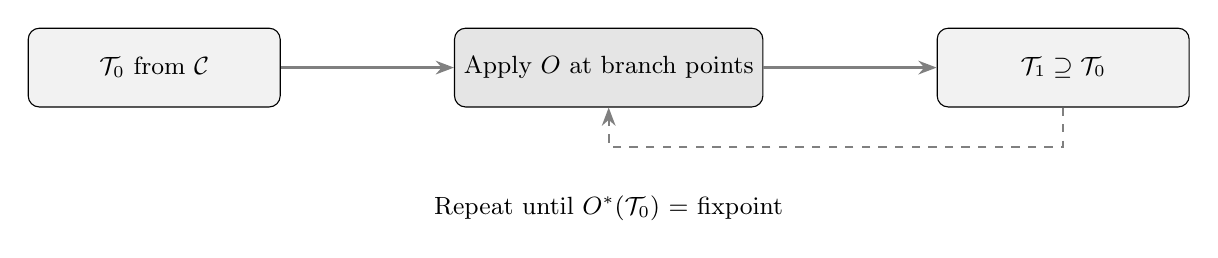
\begin{tikzpicture}[
    node distance=1.2cm,
    box/.style={draw, rounded corners, minimum width=3.2cm, minimum height=10mm, font=\small},
]
% Initial traces
\node[box, fill=black!5] (t0) {$\mathcal{T}_0$ from $\mathcal{C}$};

% Oracle application
\node[box, fill=black!10, right=2.2cm of t0] (apply) {Apply $O$ at branch points};

% New traces
\node[box, fill=black!5, right=2.2cm of apply] (t1) {$\mathcal{T}_1 \supseteq \mathcal{T}_0$};

% Fixpoint label
\node[below=1cm of apply, font=\small, align=center] {Repeat until $O^*(\mathcal{T}_0)$ = fixpoint};

% Arrows
\draw[-{Stealth}, black!50, thick] (t0) -- (apply);
\draw[-{Stealth}, black!50, thick] (apply) -- (t1);
\draw[-{Stealth}, black!50, thick, dashed] (t1.south) -- ++(0,-0.5) -| (apply.south);

\end{tikzpicture}%
}

\vspace{\vizseplg}

At fixpoint $O^*(\mathcal{T}_0)$:

\begin{itemize}
\item Every reachable HTH block has at least one exemplar trace
\item Every $R_\ell$ has been extracted via selective symbolic execution
\item The reconstructed semantics $G' = \langle X, L, \{R_\ell\}_{\ell \in L}, s_0 \rangle$ is complete
\end{itemize}

\vspace{\vizsep}
\lightrule
\vspace{\vizsep}

\subsection*{Summary: From Templates to Semantics}

\begin{enumerate}
\item \textbf{Cover} the grammar with sentinel-filled templates $\mathcal{C}$
\item \textbf{Execute} each template, recording traces at the host level
\item \textbf{Detect} HTH boundaries via sentinel appearances
\item \textbf{Extract} $R_\ell$ for each HTH region via selective symbolic execution
\item \textbf{Iterate} using the branching oracle until all reachable HTH blocks are covered
\item \textbf{Compose} the $R_\ell$ into the complete semantics $G'$
\end{enumerate}

%===============================================================================
\clearpage
\subsection*{[DRAFT] Worked Example: GCD}
%===============================================================================

% Colors by HTH block TYPE
\definecolor{hCompute}{RGB}{160, 200, 255}  % blue - computation
\definecolor{hAssign}{RGB}{255, 200, 100}   % gold - assignment
\definecolor{hControl}{RGB}{220, 180, 255}  % purple - control flow / branch
\definecolor{hSeq}{RGB}{200, 200, 200}      % gray - sequencing

\subsection*{The Algorithm}

\begin{center}
\begin{tabular}{l}
\texttt{def gcd(a, b):} \\
\texttt{1: \quad while b != 0:} \\
\texttt{2: \quad\quad t = b} \\
\texttt{3: \quad\quad b = a \% b} \\
\texttt{4: \quad\quad a = t} \\
\texttt{5: \quad return a}
\end{tabular}
\end{center}

\vspace{\vizsep}

\subsection*{Color Key by HTH Block Type}

{\small
\begin{tabular}{@{}C{1.8cm}C{1.8cm}C{1.8cm}C{1.8cm}@{}}
\colorbox{hCompute}{\,\strut Comp.\,} &
\colorbox{hAssign}{\,\strut Assign\,} &
\colorbox{hControl}{\,\strut Ctrl\,} &
\colorbox{hSeq}{\,\strut Seq\,} \\[2pt]
{\scriptsize $\ell_1$, $\ell_6$} &
{\scriptsize $\ell_4$, $\ell_7$, $\ell_9$, $\ell_{11}$} &
{\scriptsize $\ell_2$, $\ell_3$} &
{\scriptsize $\ell_5$, $\ell_8$, $\ell_{10}$}
\end{tabular}
}

\vspace{\vizsep}
\lightrule
\vspace{\vizsep}

\subsection*{HTH Blocks in This Program}

Each production's operational semantics defines jumps between holes. Every computation, every assignment, and every control flow jump is its own HTH block.

\vspace{\vizsep}

\begin{center}
\begin{tabular}{@{}cl>{\raggedright\arraybackslash}p{5.5cm}@{}}
\textbf{\#} & \textbf{Label} & \textbf{Description} \\[4pt]
\hline\\[-6pt]
1 & $\ell_1$ & \colorbox{hCompute}{compute}: b != 0 \\[4pt]
2 & $\ell_2$ & \colorbox{hControl}{control}: line 1$\to$2, enter body \\[4pt]
3 & $\ell_3$ & \colorbox{hControl}{control}: line 1$\to$5, exit loop \\[4pt]
4 & $\ell_4$ & \colorbox{hAssign}{assign}: t = b \\[4pt]
5 & $\ell_5$ & \colorbox{hSeq}{sequence}: line 2$\to$3 \\[4pt]
6 & $\ell_6$ & \colorbox{hCompute}{compute}: a \% b \\[4pt]
7 & $\ell_7$ & \colorbox{hAssign}{assign}: b = result \\[4pt]
8 & $\ell_8$ & \colorbox{hSeq}{sequence}: line 3$\to$4 \\[4pt]
9 & $\ell_9$ & \colorbox{hAssign}{assign}: a = t \\[4pt]
10 & $\ell_{10}$ & \colorbox{hSeq}{sequence}: line 4$\to$1 \\[4pt]
11 & $\ell_{11}$ & \colorbox{hAssign}{assign}: return a \\[4pt]
\end{tabular}
\end{center}

\vspace{\vizsep}

\noindent\textbf{Total: 11 unique HTH blocks.} Note that $\ell_2$ and $\ell_3$ are alternatives (branching)---only one is taken per evaluation of the condition.

%===============================================================================
\clearpage
\subsection*{[DRAFT] GCD Execution Trace: gcd(6, 4)}
%===============================================================================

\subsection*{Initial State}

$a = 6, \quad b = 4$

\vspace{\vizsep}
\lightrule
\vspace{\vizsep}

\subsection*{Loop Body Trace}

Each iteration traverses these 9 HTH blocks (values shown for both iterations):

\begin{center}
\begin{tikzpicture}[node distance=0.25cm]
% Define block style
\tikzstyle{hth}=[draw,minimum height=6mm,minimum width=14mm,font=\scriptsize]

% Vertical sequence of blocks
\node[hth,fill=hCompute] (l1) {b!=0};
\node[hth,fill=hControl,below=of l1] (l2) {line 1\textrightarrow 2};
\node[hth,fill=hAssign,below=of l2] (l4) {t=b};
\node[hth,fill=hSeq,below=of l4] (l5) {line 2\textrightarrow 3};
\node[hth,fill=hCompute,below=of l5] (l6) {a\%b};
\node[hth,fill=hAssign,below=of l6] (l7) {b=res};
\node[hth,fill=hSeq,below=of l7] (l8) {line 3\textrightarrow 4};
\node[hth,fill=hAssign,below=of l8] (l9) {a=t};
\node[hth,fill=hSeq,below=of l9] (l10) {line 4\textrightarrow 1};

% Labels on left
\node[left=0.3cm,font=\scriptsize] at (l1.west) {$\ell_1$};
\node[left=0.3cm,font=\scriptsize] at (l2.west) {$\ell_2$};
\node[left=0.3cm,font=\scriptsize] at (l4.west) {$\ell_4$};
\node[left=0.3cm,font=\scriptsize] at (l5.west) {$\ell_5$};
\node[left=0.3cm,font=\scriptsize] at (l6.west) {$\ell_6$};
\node[left=0.3cm,font=\scriptsize] at (l7.west) {$\ell_7$};
\node[left=0.3cm,font=\scriptsize] at (l8.west) {$\ell_8$};
\node[left=0.3cm,font=\scriptsize] at (l9.west) {$\ell_9$};
\node[left=0.3cm,font=\scriptsize] at (l10.west) {$\ell_{10}$};

% Arrows between blocks
\draw[-{Stealth}] (l1) -- (l2);
\draw[-{Stealth}] (l2) -- (l4);
\draw[-{Stealth}] (l4) -- (l5);
\draw[-{Stealth}] (l5) -- (l6);
\draw[-{Stealth}] (l6) -- (l7);
\draw[-{Stealth}] (l7) -- (l8);
\draw[-{Stealth}] (l8) -- (l9);
\draw[-{Stealth}] (l9) -- (l10);

% Loop back arrow
\draw[-{Stealth}] (l10.east) -- ++(0.4,0) |- ([yshift=0.15cm]l1.north east) -- (l1.north);

% Column headers
\node[right=1.0cm,font=\scriptsize\bfseries] at (l1.north east) {Iter 1};
\node[right=2.3cm,font=\scriptsize\bfseries] at (l1.north east) {Iter 2};

% Iter 1 values (right of blocks)
\node[right=1.0cm,font=\scriptsize] at (l1.east) {$4{\neq}0$ \checkmark};
\node[right=1.0cm,font=\scriptsize] at (l4.east) {$t{:=}4$};
\node[right=1.0cm,font=\scriptsize] at (l6.east) {$6\%4{=}2$};
\node[right=1.0cm,font=\scriptsize] at (l7.east) {$b{:=}2$};
\node[right=1.0cm,font=\scriptsize] at (l9.east) {$a{:=}4$};

% Iter 2 values (further right)
\node[right=2.3cm,font=\scriptsize] at (l1.east) {$2{\neq}0$ \checkmark};
\node[right=2.3cm,font=\scriptsize] at (l4.east) {$t{:=}2$};
\node[right=2.3cm,font=\scriptsize] at (l6.east) {$4\%2{=}0$};
\node[right=2.3cm,font=\scriptsize] at (l7.east) {$b{:=}0$};
\node[right=2.3cm,font=\scriptsize] at (l9.east) {$a{:=}2$};
\end{tikzpicture}
\end{center}

\noindent\textbf{State after Iter 1:} $a = 4, b = 2, t = 4$ \quad
\textbf{After Iter 2:} $a = 2, b = 0, t = 2$

\vspace{\vizsep}
\lightrule
\vspace{\vizsep}

\subsection*{Exit}

3 HTH blocks for the exit path:

\begin{center}
\begin{tikzpicture}[xscale=0.8, yscale=1.0]
\draw[thick,->] (-0.5,0) -- (10,0);

% HTH blocks colored by TYPE
\node[draw,fill=hCompute,minimum height=9mm,minimum width=14mm,font=\tiny] (neq) at (1.2,0) {b!=0};
\node[draw,fill=hControl,minimum height=9mm,minimum width=14mm,font=\tiny] (exit) at (4,0) {line 1→5};
\node[draw,fill=hAssign,minimum height=9mm,minimum width=16mm,font=\tiny] (ret) at (7,0) {return a};

\node[above=0.15cm,font=\tiny] at (neq) {$\ell_1$};
\node[above=0.15cm,font=\tiny] at (exit) {$\ell_3$};
\node[above=0.15cm,font=\tiny] at (ret) {$\ell_{11}$};

\node[below=0.35cm,font=\tiny,align=center] at (neq) {0$\neq$0\\false};
\node[below=0.35cm,font=\tiny] at (exit) {exit loop};
\node[below=0.35cm,font=\tiny] at (ret) {returns 2};
\end{tikzpicture}
\end{center}

\noindent\textbf{Result:} $\text{gcd}(6, 4) = 2$

%===============================================================================
\clearpage
\subsection*{[DRAFT] GCD: The Complete HTH Graph}
%===============================================================================

\subsection*{All 11 HTH Blocks}

The HTH blocks form a graph. Loops create cycles; branches create forks.

\vspace{\vizsep}

\noindent\resizebox{\columnwidth}{!}{%
\begin{tikzpicture}[
    node distance=0.7cm and 1.2cm,
    block/.style={draw, rounded corners, minimum width=1.2cm, minimum height=6mm, font=\scriptsize},
    every edge/.style={draw, -{Stealth}, black!60}
]

% Main flow - colored by TYPE
\node[block, fill=hCompute] (neq) {$\ell_1$: b!=0};
\node[block, fill=hControl, above right=0.5cm and 1.2cm of neq] (enter) {$\ell_2$: line 1→2};
\node[block, fill=hControl, below right=0.8cm and 1.2cm of neq] (exit) {$\ell_3$: line 1→5};
\node[block, fill=hAssign, right=of enter] (t) {$\ell_4$: t=b};
\node[block, fill=hSeq, right=of t] (s1) {$\ell_5$: line 2→3};
\node[block, fill=hCompute, right=of s1] (mod) {$\ell_6$: a\%b};
\node[block, fill=hAssign, below=of mod] (b) {$\ell_7$: b=res};
\node[block, fill=hSeq, left=of b] (s2) {$\ell_8$: line 3→4};
\node[block, fill=hAssign, left=of s2] (a) {$\ell_9$: a=t};
\node[block, fill=hSeq, left=1cm of a] (loop) {$\ell_{10}$: line 4→1};
\node[block, fill=hAssign, below=of exit] (ret) {$\ell_{11}$: ret};

% Edges
\draw[->] (neq) -- (enter) node[midway, above, font=\tiny] {true};
\draw[->] (neq) -- (exit) node[midway, below, font=\tiny] {false};
\draw[->] (enter) -- (t);
\draw[->] (t) -- (s1);
\draw[->] (s1) -- (mod);
\draw[->] (mod) -- (b);
\draw[->] (b) -- (s2);
\draw[->] (s2) -- (a);
\draw[->] (a) -- (loop);
\draw[->] (loop.west) to[out=180, in=-90] (neq.south);
\draw[->] (exit) -- (ret);

\end{tikzpicture}%
}

\vspace{\vizsep}

\subsection*{Relational Transformers (all 11)}

{\small
\begin{align*}
R_{\ell_1} &:= x'[\text{cmp}] = (x[\text{b}] \neq 0) \\
R_{\ell_2} &:= x[\text{cmp}] \land x' = x \\
R_{\ell_3} &:= \neg x[\text{cmp}] \land x' = x \\
R_{\ell_4} &:= x'[\text{t}] = x[\text{b}] \\
R_{\ell_5} &:= x' = x \\
R_{\ell_6} &:= x'[\text{tmp}] = x[\text{a}] \mathbin{\%} x[\text{b}] \\
R_{\ell_7} &:= x'[\text{b}] = x[\text{tmp}] \\
R_{\ell_8} &:= x' = x \\
R_{\ell_9} &:= x'[\text{a}] = x[\text{t}] \\
R_{\ell_{10}} &:= x' = x \\
R_{\ell_{11}} &:= x'[\text{ret}] = x[\text{a}]
\end{align*}
}

\vspace{\vizsep}
\lightrule
\vspace{\vizsep}

\subsection*{Key Observations}

\begin{itemize}
\item \textbf{Same HTH blocks, different values:} Iterations 1 and 2 traverse the \emph{same} 9 HTH blocks ($\ell_1, \ell_2, \ell_4, \ell_5, \ell_6, \ell_7, \ell_8, \ell_9, \ell_{10}$) but with different concrete values. The HTH blocks are the \emph{schema}; the values are the \emph{instantiation}.

\item \textbf{Every step is an HTH block:} Computations ($\ell_1$, $\ell_6$), assignments ($\ell_4$, $\ell_7$, $\ell_9$), control flow jumps ($\ell_2$, $\ell_3$, $\ell_{10}$), and sequencing ($\ell_5$, $\ell_8$) are \emph{all} HTH blocks. There is no distinction---evaluation order \emph{is} the sequence of HTH blocks.

\item \textbf{Branching creates alternatives:} $\ell_2$ (enter body) and $\ell_3$ (exit loop) are alternatives at the same branch point. Their guards are mutually exclusive: $x[\text{cmp}] = \text{true}$ vs $x[\text{cmp}] = \text{false}$.

\item \textbf{The loop is a cycle:} $\ell_{10}$ (loop back) connects the end of the body back to $\ell_1$ (condition), creating a cycle in the HTH graph.

\item \textbf{Composition gives semantics:} The full GCD semantics is the composition of these 11 $R_\ell$ along all paths through the HTH graph.
\end{itemize}

%===============================================================================
\clearpage
\subsection*{[DRAFT] Synthesis: HTH-Based Semantics Extraction}
%===============================================================================

This section integrates all visualizations to show how we extract executable semantics from interpreter traces.

\subsection*{Core Concept: HTH Blocks}

A \textbf{Hole-to-Hole (HTH) block} is an atomic unit of semantic behavior---the smallest step the interpreter takes between observable points. Every program execution is a sequence of HTH blocks.

\vspace{\vizsep}

\noindent\textbf{The four types of HTH blocks:}

\begin{center}
{\small
\begin{tabular}{@{}C{1.7cm}C{1.7cm}C{1.7cm}C{1.7cm}@{}}
\colorbox{hCompute}{\,\strut Compute\,} &
\colorbox{hAssign}{\,\strut Assign\,} &
\colorbox{hControl}{\,\strut Control\,} &
\colorbox{hSeq}{\,\strut Sequence\,} \\[4pt]
{\footnotesize evaluates} &
{\footnotesize stores} &
{\footnotesize branches} &
{\footnotesize advances} \\
{\footnotesize expressions} &
{\footnotesize results} &
{\footnotesize on condition} &
{\footnotesize to next stmt}
\end{tabular}
}
\end{center}

\vspace{\vizsep}

\noindent\textbf{Example:} For \texttt{gcd(a, b)}, the statement \texttt{b = a \% b} decomposes into:

\begin{center}
\begin{tikzpicture}[node distance=0.3cm]
\tikzstyle{hth}=[draw,minimum height=6mm,minimum width=16mm,font=\scriptsize]
\node[hth,fill=hCompute] (comp) {a\%b};
\node[hth,fill=hAssign,right=0.8cm of comp] (asgn) {b=result};
\node[hth,fill=hSeq,right=0.8cm of asgn] (seq) {line 3\textrightarrow 4};
\draw[-{Stealth}] (comp) -- (asgn);
\draw[-{Stealth}] (asgn) -- (seq);
\node[above=2pt,font=\tiny] at (comp.north) {$\ell_6$};
\node[above=2pt,font=\tiny] at (asgn.north) {$\ell_7$};
\node[above=2pt,font=\tiny] at (seq.north) {$\ell_8$};
\end{tikzpicture}
\end{center}

\vspace{\vizsep}
\lightrule
\vspace{\vizsep}

\subsection*{From Traces to Relational Transformers}

Each HTH block $\ell$ has an associated \textbf{relational transformer} $R_\ell(x, x')$ that relates the input configuration $x$ to the output configuration $x'$:
\[
R_\ell(x, x') \;:=\; \text{Guard}_\ell(x) \;\land\; \text{Update}_\ell(x, x')
\]

\begin{itemize}
\item \textbf{Guard}: Under what conditions is this block taken?
\item \textbf{Update}: How does the state change?
\end{itemize}

\vspace{\vizsep}
\lightrule
\vspace{\vizsep}

\subsection*{Complete Example: GCD}

\noindent\textbf{The algorithm:}
\begin{center}
\begin{tabular}{l}
\texttt{def gcd(a, b):} \\
\texttt{1: \quad while b != 0:} \\
\texttt{2: \quad\quad t = b} \\
\texttt{3: \quad\quad b = a \% b} \\
\texttt{4: \quad\quad a = t} \\
\texttt{5: \quad return a}
\end{tabular}
\end{center}

\vspace{\vizsep}

\noindent\textbf{The HTH graph} shows all 11 blocks and their connections. Loops create cycles; branches create forks:

\begin{center}
\begin{tikzpicture}[
    node distance=0.4cm and 0.7cm,
    block/.style={draw, rounded corners, minimum width=1.0cm, minimum height=5mm, font=\tiny},
    every edge/.style={draw, -{Stealth}, black!60}
]
% Main flow
\node[block, fill=hCompute] (neq) {$\ell_1$: b!=0};
\node[block, fill=hControl, above right=0.35cm and 0.7cm of neq] (enter) {$\ell_2$: 1\textrightarrow 2};
\node[block, fill=hControl, below right=0.5cm and 0.7cm of neq] (exit) {$\ell_3$: 1\textrightarrow 5};
\node[block, fill=hAssign, right=of enter] (t) {$\ell_4$: t=b};
\node[block, fill=hSeq, right=of t] (s1) {$\ell_5$};
\node[block, fill=hCompute, right=of s1] (mod) {$\ell_6$: a\%b};
\node[block, fill=hAssign, below=of mod] (b) {$\ell_7$: b=r};
\node[block, fill=hSeq, left=of b] (s2) {$\ell_8$};
\node[block, fill=hAssign, left=of s2] (a) {$\ell_9$: a=t};
\node[block, fill=hSeq, left=0.5cm of a] (loop) {$\ell_{10}$};
\node[block, fill=hAssign, below=of exit] (ret) {$\ell_{11}$: ret};

\draw[->] (neq) -- (enter) node[midway, above, font=\tiny] {T};
\draw[->] (neq) -- (exit) node[midway, below, font=\tiny] {F};
\draw[->] (enter) -- (t);
\draw[->] (t) -- (s1);
\draw[->] (s1) -- (mod);
\draw[->] (mod) -- (b);
\draw[->] (b) -- (s2);
\draw[->] (s2) -- (a);
\draw[->] (a) -- (loop);
\draw[->] (loop.west) to[out=180, in=-90] (neq.south);
\draw[->] (exit) -- (ret);
\end{tikzpicture}
\end{center}

\vspace{\vizsep}

\noindent\textbf{Execution trace for gcd(6, 4):} Two loop iterations, then exit.

\begin{center}
\begin{tikzpicture}[node distance=0.22cm]
\tikzstyle{hth}=[draw,minimum height=5.5mm,minimum width=13mm,font=\tiny]

% Vertical sequence
\node[hth,fill=hCompute] (l1) {b!=0};
\node[hth,fill=hControl,below=of l1] (l2) {line 1\textrightarrow 2};
\node[hth,fill=hAssign,below=of l2] (l4) {t=b};
\node[hth,fill=hSeq,below=of l4] (l5) {line 2\textrightarrow 3};
\node[hth,fill=hCompute,below=of l5] (l6) {a\%b};
\node[hth,fill=hAssign,below=of l6] (l7) {b=res};
\node[hth,fill=hSeq,below=of l7] (l8) {line 3\textrightarrow 4};
\node[hth,fill=hAssign,below=of l8] (l9) {a=t};
\node[hth,fill=hSeq,below=of l9] (l10) {line 4\textrightarrow 1};

% Labels
\node[left=0.25cm,font=\tiny] at (l1.west) {$\ell_1$};
\node[left=0.25cm,font=\tiny] at (l2.west) {$\ell_2$};
\node[left=0.25cm,font=\tiny] at (l4.west) {$\ell_4$};
\node[left=0.25cm,font=\tiny] at (l5.west) {$\ell_5$};
\node[left=0.25cm,font=\tiny] at (l6.west) {$\ell_6$};
\node[left=0.25cm,font=\tiny] at (l7.west) {$\ell_7$};
\node[left=0.25cm,font=\tiny] at (l8.west) {$\ell_8$};
\node[left=0.25cm,font=\tiny] at (l9.west) {$\ell_9$};
\node[left=0.25cm,font=\tiny] at (l10.west) {$\ell_{10}$};

% Arrows
\draw[-{Stealth}] (l1) -- (l2);
\draw[-{Stealth}] (l2) -- (l4);
\draw[-{Stealth}] (l4) -- (l5);
\draw[-{Stealth}] (l5) -- (l6);
\draw[-{Stealth}] (l6) -- (l7);
\draw[-{Stealth}] (l7) -- (l8);
\draw[-{Stealth}] (l8) -- (l9);
\draw[-{Stealth}] (l9) -- (l10);
\draw[-{Stealth}] (l10.east) -- ++(0.35,0) |- ([yshift=0.12cm]l1.north east) -- (l1.north);

% Headers
\node[right=0.7cm,font=\tiny\bfseries] at (l1.north east) {Iter 1};
\node[right=1.7cm,font=\tiny\bfseries] at (l1.north east) {Iter 2};

% Iter 1 values
\node[right=0.7cm,font=\tiny] at (l1.east) {$4{\neq}0$};
\node[right=0.7cm,font=\tiny] at (l4.east) {$t{:=}4$};
\node[right=0.7cm,font=\tiny] at (l6.east) {$6\%4{=}2$};
\node[right=0.7cm,font=\tiny] at (l7.east) {$b{:=}2$};
\node[right=0.7cm,font=\tiny] at (l9.east) {$a{:=}4$};

% Iter 2 values
\node[right=1.7cm,font=\tiny] at (l1.east) {$2{\neq}0$};
\node[right=1.7cm,font=\tiny] at (l4.east) {$t{:=}2$};
\node[right=1.7cm,font=\tiny] at (l6.east) {$4\%2{=}0$};
\node[right=1.7cm,font=\tiny] at (l7.east) {$b{:=}0$};
\node[right=1.7cm,font=\tiny] at (l9.east) {$a{:=}2$};

% Exit path (to the right)
\node[right=3.5cm,font=\tiny\bfseries] at (l1.east) {Exit};
\node[hth,fill=hCompute,right=3.5cm] at (l1.east) (e1) {b!=0};
\node[hth,fill=hControl,below=of e1] (e3) {line 1\textrightarrow 5};
\node[hth,fill=hAssign,below=of e3] (e11) {return a};

\node[left=0.15cm,font=\tiny] at (e1.west) {$\ell_1$};
\node[left=0.15cm,font=\tiny] at (e3.west) {$\ell_3$};
\node[left=0.15cm,font=\tiny] at (e11.west) {$\ell_{11}$};

\draw[-{Stealth}] (e1) -- (e3);
\draw[-{Stealth}] (e3) -- (e11);

\node[right=0.3cm,font=\tiny] at (e1.east) {$0{\neq}0$ false};
\node[right=0.3cm,font=\tiny] at (e11.east) {ret 2};

\end{tikzpicture}
\end{center}

\vspace{\vizsep}

\noindent\textbf{Key insight:} Both iterations traverse the \emph{same} 9 HTH blocks with \emph{different} values. The blocks are the \textbf{schema}; the values are the \textbf{instantiation}. This is why we can extract a single set of relational transformers that work for all inputs.

\vspace{\vizsep}
\lightrule
\vspace{\vizsep}

\subsection*{The Extracted Semantics}

The relational transformers, composed along paths through the HTH graph, give us the complete operational semantics:

{\small
\begin{align*}
R_{\ell_1} &:= x'[\text{cmp}] = (x[\text{b}] \neq 0) & \text{(compute condition)} \\
R_{\ell_2} &:= x[\text{cmp}] \land x' = x & \text{(enter body if true)} \\
R_{\ell_3} &:= \neg x[\text{cmp}] \land x' = x & \text{(exit loop if false)} \\
R_{\ell_4} &:= x'[\text{t}] = x[\text{b}] & \text{(save b to t)} \\
R_{\ell_6} &:= x'[\text{r}] = x[\text{a}] \mathbin{\%} x[\text{b}] & \text{(compute remainder)} \\
R_{\ell_7} &:= x'[\text{b}] = x[\text{r}] & \text{(update b)} \\
R_{\ell_9} &:= x'[\text{a}] = x[\text{t}] & \text{(update a)} \\
R_{\ell_{11}} &:= x'[\text{ret}] = x[\text{a}] & \text{(return result)}
\end{align*}
}

\noindent(Sequence blocks $\ell_5, \ell_8, \ell_{10}$ have $R_\ell := x' = x$---they advance control without changing state.)

\vspace{\vizsep}
\lightrule
\vspace{\vizsep}

\subsection*{From Programs to Languages}

GCD is a worked example, but our goal is extracting \textbf{language semantics}, not program semantics. The covering set $\mathcal{C}$ contains templates that exercise every grammar production---not every program.

\vspace{\vizsep}

\noindent\textbf{Covering sets and control flow.} For a production like \texttt{if-then-else}, the covering set includes templates where the condition hole is filled with:
\begin{itemize}
\item \textbf{Low-cardinality types}: All values exhaustively (e.g., \texttt{True}, \texttt{False})
\item \textbf{High-frequency literals}: Common values like \texttt{0}, \texttt{1}, \texttt{-1}, \texttt{None}, \texttt{""}, \texttt{[]}
\end{itemize}
These first-round traces already exercise both branches for simple conditions. The branching oracle handles computed/complex conditions.

\vspace{\vizsep}

\noindent\textbf{Truthiness and method dispatch.} In Python, \texttt{if x:} doesn't compare \texttt{x} to \texttt{True}---it calls \texttt{x.\_\_bool\_\_()}. How do we capture this?

Because we trace at the \emph{interpreter level}, method dispatch is visible. The HTH decomposition for \texttt{if cond:} is not a single ``evaluate and branch'' block, but a sequence:

\begin{center}
\begin{tikzpicture}[node distance=0.2cm]
\tikzstyle{hth}=[draw,minimum height=5mm,minimum width=15mm,font=\tiny]
\node[hth,fill=hCompute] (eval) {eval cond};
\node[hth,fill=gray!20,right=0.5cm of eval] (bool) {.\_\_bool\_\_()};
\node[hth,fill=hControl,right=0.5cm of bool] (branch) {branch};
\draw[-{Stealth}] (eval) -- (bool);
\draw[-{Stealth}] (bool) -- (branch);
\node[above=1pt,font=\tiny] at (eval.north) {yields $v$};
\node[above=1pt,font=\tiny] at (bool.north) {dispatch};
\node[above=1pt,font=\tiny] at (branch.north) {T/F};
\end{tikzpicture}
\end{center}

The \texttt{\_\_bool\_\_} call is just more HTH blocks. We see it in the trace because function entry/exit are observable points. The covering set for \texttt{\_\_bool\_\_}'s return type is trivially $\{\texttt{True}, \texttt{False}\}$, giving us branch coverage automatically.

\vspace{2pt}
\noindent\textit{Method dispatch isn't special---it's HTH blocks all the way down.}

\vspace{\vizsep}
\lightrule
\vspace{\vizsep}

\subsection*{Summary: The Extraction Pipeline}

\begin{enumerate}
\item \textbf{Execute} the interpreter on test inputs, recording traces
\item \textbf{Detect} HTH block boundaries via sentinel values
\item \textbf{Segment} traces into HTH regions
\item \textbf{Extract} $R_\ell$ for each block via selective symbolic execution
\item \textbf{Compose} the $R_\ell$ along the HTH graph to get full semantics
\end{enumerate}

The result is a \textbf{labeled transition system} that simulates the original interpreter---same observable behavior, but now we have explicit, composable semantic rules. (With exact symbolic execution, bisimulation among reachable states; see Remarks.)

%===============================================================================
\clearpage
\subsection*{[DRAFT] Covering Set Examples (Python)}
%===============================================================================

A \textbf{covering set} $\mathcal{C}$ contains template programs that exercise every grammar production. Each template has \textbf{sentinel holes} filled with values chosen to maximize behavioral coverage. Below are concrete examples for several Python productions.

\vspace{\vizsep}
\lightrule
\vspace{\vizsep}

\subsection*{1. If-Then-Else}

\noindent\textbf{Production:} \texttt{stmt ::= 'if' expr ':' suite ('else' ':' suite)?}

\noindent\textbf{Holes:} condition expression, then-body, else-body

\noindent\textbf{Covering set templates:}
\begin{lstlisting}
if True:  x = 1      # cond = True
else:     x = 2

if False: x = 1      # cond = False
else:     x = 2

if 0:     x = 1      # cond = 0 (falsy int)
else:     x = 2

if 1:     x = 1      # cond = 1 (truthy int)
else:     x = 2

if []:    x = 1      # cond = [] (falsy list)
else:     x = 2

if None:  x = 1      # cond = None
else:     x = 2
\end{lstlisting}

\noindent\textit{These exercise both branches and reveal truthiness for multiple types.}

\vspace{\vizsep}
\lightrule
\vspace{\vizsep}

\subsection*{2. While Loop}

\noindent\textbf{Production:} \texttt{stmt ::= 'while' expr ':' suite}

\noindent\textbf{Holes:} condition expression, loop body

\noindent\textbf{Covering set templates:}
\begin{lstlisting}
while False: x = 1   # cond false: skip body

while True:          # cond true: enter body
    x = 1
    break
\end{lstlisting}

\noindent\textit{Just two templates suffice! We see all HTH transitions: condition eval, true/false guards, body entry, exit. The ``loop back'' edge is structural---we don't need multiple iterations to learn it.}

\vspace{\vizsep}
\lightrule
\vspace{\vizsep}

\subsection*{3. Binary Arithmetic (\texttt{+})}

\noindent\textbf{Production:} \texttt{expr ::= expr '+' expr}

\noindent\textbf{Holes:} left operand, right operand

\noindent\textbf{Covering set templates:}
\begin{lstlisting}
x = 1 + 2            # int addition
x = "a" + "b"        # string concat
x = [1] + [2]        # list concat
\end{lstlisting}

\noindent\textit{Key insight: these produce \textbf{different HTH traces}! Each type dispatches to its own \texttt{\_\_add\_\_}. Concrete execution reveals this polymorphism directly---no type system modeling required.}

\vspace{\vizsep}
\lightrule
\vspace{\vizsep}

\subsection*{4. Indexing}

\noindent\textbf{Production:} \texttt{expr ::= expr '[' expr ']'}

\noindent\textbf{Holes:} container, index

\noindent\textbf{Covering set templates:}
\begin{lstlisting}
x = [10, 20, 30][0]   # list, first
x = [10, 20, 30][-1]  # list, negative
x = {"a": 1}["a"]     # dict
x = "hello"[0]        # string
\end{lstlisting}

\noindent\textit{The container hole is filled from \texttt{expr}'s covering set, which includes various types. This reveals type-specific \texttt{\_\_getitem\_\_} dispatch.}

\vspace{\vizsep}
\lightrule
\vspace{\vizsep}

\subsection*{5. Function Definition and Call}

\noindent\textbf{Productions:}
\begin{itemize}
\item \texttt{stmt ::= 'def' NAME '(' params ')' ':' suite}
\item \texttt{expr ::= NAME '(' args ')'}
\end{itemize}

\noindent\textbf{Covering set templates:}
\begin{lstlisting}
def f(): return 1     # 0-arity
x = f()

def g(a): return a    # 1-arity
x = g(42)

def h(a, b):          # 2-arity
    return a + b
x = h(1, 2)

def k(a=10): return a # default arg
x = k()
x = k(20)
\end{lstlisting}

\noindent\textit{Exercises function entry/exit, argument passing, defaults.}

\vspace{\vizsep}
\lightrule
\vspace{\vizsep}

\subsection*{6. Attribute Access}

\noindent\textbf{Production:} \texttt{expr ::= expr '.' NAME}

\noindent\textbf{Holes:} object, attribute name

\noindent\textbf{Covering set templates:}
\begin{lstlisting}
class C:
    x = 10
    def m(self): return 1

obj = C()
y = obj.x             # attr read
z = obj.m()           # method call
obj.x = 20            # attr write
\end{lstlisting}

\noindent\textit{Reveals \texttt{\_\_getattr\_\_}/\texttt{\_\_setattr\_\_} and method binding.}

\vspace{\vizsep}
\lightrule
\vspace{\vizsep}

\subsection*{7. For Loop}

\noindent\textbf{Production:} \texttt{stmt ::= 'for' NAME 'in' expr ':' suite}

\noindent\textbf{Holes:} loop variable, iterable, body

\noindent\textbf{Covering set templates:}
\begin{lstlisting}
for x in []: y = x      # empty (0 iters)
for x in [1]: y = x     # single element
for x in [1,2]: y = x   # multiple
for x in "ab": y = x    # string iter
\end{lstlisting}

\noindent\textit{Exercises iterator protocol (\texttt{\_\_iter\_\_}, \texttt{\_\_next\_\_}).}

\vspace{\vizsep}
\lightrule
\vspace{\vizsep}

\subsection*{8. Try-Except}

\noindent\textbf{Production:} \texttt{stmt ::= 'try' ':' suite 'except' ... ':' suite}

\noindent\textbf{Covering set templates:}
\begin{lstlisting}
try:               # no exception
    x = 1
except:
    x = 2

try:               # exception raised
    x = 1 / 0
except:
    x = 2

try:               # typed exception
    x = int("bad")
except ValueError:
    x = 0
\end{lstlisting}

\noindent\textit{Exercises normal completion, exception raise, exception matching.}

\vspace{\vizsep}
\lightrule
\vspace{\vizsep}

\subsection*{Summary}

Each production's covering set is designed to:
\begin{enumerate}
\item Exercise all control flow paths (branches, iterations, exceptions)
\item Include boundary values (0, 1, -1, empty, single-element)
\item Reveal type-dependent dispatch (\texttt{\_\_add\_\_}, \texttt{\_\_bool\_\_}, etc.)
\item Cover literals that trigger special behavior
\end{enumerate}

The union of all production covering sets forms $\mathcal{C}$. Executing these generates traces that, segmented into HTH blocks, yield the complete language semantics.

\vspace{\vizsep}

\noindent\textbf{Why concrete execution first?} Two reasons:
\begin{enumerate}
\item \textbf{Boundary detection}: Sentinel values in traces let us \emph{find} HTH block boundaries empirically. The grammar tells us syntactic structure, but not evaluation order or implicit dispatches.
\item \textbf{Type dispatch discovery}: Different types produce different traces for the same production (e.g., \texttt{+} on ints vs strings). Concrete execution reveals this polymorphism without modeling the type system.
\end{enumerate}
After boundary detection, we use selective symbolic execution to generalize each HTH segment into its relational transformer $R_\ell$.

%===============================================================================
\clearpage
\subsection*{Algorithm 1: Syntax-Only Covering Set Generation}
%===============================================================================

\noindent\textbf{Reference:} tree-sitter-python \texttt{grammar.js}

\vspace{0.5em}
\noindent\textbf{Input:} A grammar production $P$

\vspace{0.5em}
\noindent\textbf{For each production $P$:}

\begin{enumerate}
\item \textbf{Identify holes}---the field positions referencing other rules.

Example for \texttt{if\_statement}:
\begin{lstlisting}[basicstyle=\ttfamily\small]
if_statement: $ => seq(
  'if',
  field('condition', $.expression),
  ':',
  field('consequence', $.block),
  optional(field('alternative', $.else_clause)),
)
\end{lstlisting}

\begin{center}
\begin{tabular}{ll}
\toprule
\textbf{Field} & \textbf{Sort} \\
\midrule
\texttt{condition} & \texttt{expression} \\
\texttt{consequence} & \texttt{block} \\
\texttt{alternative} & \texttt{else\_clause} (optional) \\
\bottomrule
\end{tabular}
\end{center}

\item \textbf{Generate minimal fillers} for each sort:

\begin{center}
\footnotesize
\begin{tabular}{lp{5.5cm}}
\toprule
\textbf{Sort} & \textbf{Minimal Fillers} \\
\midrule
\texttt{expression} & \texttt{0}, \texttt{1}, \texttt{""}, \texttt{"x"}, \texttt{True}, \texttt{False}, \texttt{None}, \texttt{[]}, \texttt{[1]} \\
\texttt{block} & \texttt{pass}, \texttt{x = 1} \\
\texttt{identifier} & \texttt{f} (fresh) \\
\texttt{integer} & \texttt{0}, \texttt{1}, \texttt{-1} \\
\texttt{string} & \texttt{""}, \texttt{"x"} \\
\texttt{list} & \texttt{[]}, \texttt{[1]}, \texttt{[1, 2]} \\
\bottomrule
\end{tabular}
\end{center}

\item \textbf{Combine} to create covering templates:

\begin{lstlisting}
if 0: pass          # falsy integer
if 1: pass          # truthy integer
if "": pass         # falsy string
if "x": pass        # truthy string
if []: pass         # falsy list
if [1]: pass        # truthy list
if None: pass       # None (falsy)
if True: pass       # bool True
if False: pass      # bool False
\end{lstlisting}

\end{enumerate}

\noindent\textbf{Output:} Set of syntactically valid programs covering production $P$.

%===============================================================================
\clearpage
\subsection*{Algorithm 2: Identifier Resolution Discovery}
%===============================================================================

\noindent\textbf{Reference:} tree-sitter-python \texttt{grammar.js}

\vspace{0.5em}
\noindent\textbf{Input:} Grammar $G$, token \texttt{identifier}

\vspace{0.5em}
\noindent\textbf{Step 1: Collect identifier-containing productions}

\begin{center}
\footnotesize
\begin{tabular}{llr}
\toprule
\textbf{Production} & \textbf{Identifier Field} & \textbf{Role} \\
\midrule
\texttt{function\_definition} & \texttt{name} & binder \\
\texttt{class\_definition} & \texttt{name} & binder \\
\texttt{assignment} & \texttt{left} & binder \\
\texttt{primary\_expression} & (direct) & reference \\
\texttt{call} & \texttt{function} & reference \\
\texttt{attribute} & \texttt{attribute} & reference \\
\texttt{global\_statement} & (direct) & scope mod \\
\texttt{nonlocal\_statement} & (direct) & scope mod \\
\bottomrule
\end{tabular}
\end{center}

\vspace{0.5em}
\noindent\textbf{Step 2: Generate single-identifier test programs}

Using fresh identifier \texttt{f}:

\begin{lstlisting}
f                     # primary_expression (reference)
f()                   # call (reference)
f = 1                 # assignment (binder)
def f(): pass         # function_definition (binder)
class f: pass         # class_definition (binder)
\end{lstlisting}

\vspace{0.5em}
\noindent\textbf{Step 3: Execute and record outcomes}

\begin{center}
\begin{tabular}{ll}
\toprule
\textbf{Test Program} & \textbf{Outcome} \\
\midrule
\texttt{f} & \texttt{NameError} \\
\texttt{f()} & \texttt{NameError} \\
\texttt{f = 1} & OK \\
\texttt{def f(): pass} & OK \\
\texttt{class f: pass} & OK \\
\texttt{f = 1; f} & OK \\
\texttt{def f(): pass; f()} & OK \\
\texttt{f = 1; f()} & \texttt{TypeError} \\
\texttt{def f(): pass; f = 1; f()} & \texttt{TypeError} \\
\bottomrule
\end{tabular}
\end{center}

\vspace{0.5em}
\noindent\textbf{Step 4: Infer structure}

\begin{itemize}
\item \textbf{Binders}: \texttt{function\_definition}, \texttt{class\_definition}, \texttt{assignment}
\item \textbf{References}: \texttt{identifier} (in \texttt{primary\_expression}), \texttt{call}
\item \textbf{Ordering constraint}: binder $\prec$ reference
\item \textbf{Namespace}: unified (function/class/variable share namespace, can shadow)
\item \textbf{Type dispatch}: \texttt{call} requires callable value
\end{itemize}

\vspace{0.5em}
\noindent\textbf{Output:}
\begin{itemize}
\item Binder/reference classification per production
\item Ordering constraints (binding must precede reference)
\item Namespace structure (unified vs.\ separate)
\end{itemize}

%===============================================================================
\clearpage
\subsection*{Key tree-sitter-python Sorts}
%===============================================================================

\begin{center}
\footnotesize
\begin{tabular}{lp{4.3cm}}
\toprule
\textbf{Sort} & \textbf{Description} \\
\midrule
\texttt{identifier} & Name token \\
\texttt{expression} & Any expression \\
\texttt{primary\_expression} & Atomic: id, literals, call, subscript, attr \\
\texttt{block} & Indented body \\
\texttt{call} & Function/method call \\
\texttt{subscript} & Indexing \texttt{x[i]} \\
\texttt{attribute} & Attribute access \texttt{x.y} \\
\texttt{assignment} & Binding \texttt{x = e} \\
\texttt{function\_definition} & \texttt{def f(): block} \\
\texttt{class\_definition} & \texttt{class C: block} \\
\texttt{if\_statement} & \texttt{if cond: block} \\
\texttt{while\_statement} & \texttt{while cond: block} \\
\texttt{for\_statement} & \texttt{for x in e: block} \\
\texttt{integer} & Integer literal \\
\texttt{string} & String literal \\
\texttt{list} & List literal \texttt{[...]} \\
\texttt{true}/\texttt{false}/\texttt{none} & Boolean/None literals \\
\bottomrule
\end{tabular}
\end{center}

\end{document}
